\setchapterimage{model-6}
\setchapterpreamble[u]{\margintoc}
\chapter{Model description}\labch{Chapter2}
\label{Chapter2} % For referencing the chapter elsewhere, use \ref{Chapter2} 
\section{Introduction}
This Chapter describes the mathematical models needed to simulate H transport in tokamaks plasma facing components.
The numerical scheme to solve these equations and an introduction to the finite element method alongside with its implementation in the FESTIM code are also presented.
Finally, the verification \& validation of FESTIM is performed to guaranty its reliability.

\section{H transport} \label{description_H_transport_model}

This Section describes the main model for simulating H transport in materials.

\subsection{Macroscopic Rate Equations model}

The Macroscopic Rate Equations (MRE) model will be employed.
The principle is to split the hydrogen isotopes into several populations: the mobile hydrogen particles and the hydrogen particles trapped in the i-th trap.
Their concentration in \si{H.m^{-3}} are respectively $c_\mathrm{m}$ and $c_{\mathrm{t},i}$.
They can be expressed in atomic fraction (at.fr.) by normalising them to the atomic density of the material.

Fick's first law of diffusion states that the particle flux is driven by the concentration gradient.
The particle flux $J$ is therefore expressed by:
\begin{equation}
    J = - D \nabla c_\mathrm{m}
\end{equation}
where $D$ is the diffusion coefficient in \si{m^2.s^{-1}}.
This expression neglects the Soret effect or the effect of hydrostatic pressure.

% This particle flux can be expressed differently if additionnal physics are accounted for.
% For instance, taking into account the Soret effect (also called thermodiffusion or thermophoresis), the particle flux is expressed as:
% \begin{equation}
%     J = - D \nabla c_\mathrm{m} - D \frac{c_\mathrm{m} Q}{R T^2} \nabla T
% \end{equation}
% where $Q$ is the Soret coefficient (or heat of transport) expressed in \si{J.mol^{-1}}, $T$ is the temperature in \si{K} and $R=\SI{8.314}{J.mol^{-1}.K^{-1}}$ is the gas constant.
% This effect will enhance the diffusion when particles diffuse from a hot region to a cold region.
% It should be noted however that the Soret coefficient is fairly difficult to measure.

The spatio-temporal evolution of these concentrations is commonly described by the following reaction-diffusion system:

\begin{equation}
    \frac{\partial c_\mathrm{m}}{\partial t}=\nabla \cdot J+\Gamma-\sum \frac{\partial c_{\mathrm{t}, i}}{\partial t}
    \label{eq:mobile}
\end{equation}

\begin{equation}
    \frac{\partial c_{\mathrm{t}, i}}{\partial t}=k \cdot c_\mathrm{m} \cdot\left(n_{i}-c_{\mathrm{t}, i}\right)-p \cdot c_{\mathrm{t}, i}
    \label{eq:trapped}
\end{equation}

In Equation \ref{eq:mobile}, $\Gamma$ is the volumetric source term of particles in \si{m^{-3}.s^{-1}}.
The volumetric source term can be used to simulate any process producing H in the bulk.
This is the case for plasma implantation and nuclear reactions producing H.

In Equation \ref{eq:trapped}, $k$ and $p$ are the trapping and detrapping rates expressed in \si{m^3.s^{-1}} and \si{s^{-1}} respectively and $n_i$ is the trap density in \si{m^{-3}}.

At steady state (\textit{ie} $\frac{\partial c_\mathrm{m}}{\partial t} = 0$ and $\frac{\partial c_{\mathrm{t}, i}}{\partial t} = 0$), the mobile H concentration is independent of $c_{\mathrm{t}, i}$.
Equation \ref{eq:trapped} can be rewritten as:
\begin{equation}
    c_{\mathrm{t}, i} = n_i \frac{1}{\frac{p}{k c_\mathrm{m}} + 1}
    \label{eq: steady state ct}
\end{equation}
The quantity $(p / (k c_\mathrm{m}) + 1)^{-1}$ determines the filling ratio of the trap. 
As it approaches one (high mobile concentration, low detrapping rate or high trapping rate), the trapped concentration approaches the trap density.
As it approaches zero (high detrapping rate, low mobile concentration or low trapping rate), the trapped concentration approaches zero.

\subsection{Boundary conditions}

Several boundary conditions will be employed in order to constrain either the concentration (Dirichlet boundary condition) or the concentration gradient (Neumann, Robin boundary condition) at the domain's boundaries.

\subsubsection{Dissociation and recombination fluxes}

The concentration gradient can also be constrained on the boundaries (see Equation \ref{eq: neuman robin bc}).

\begin{equation}
    - D(T)\nabla c_\mathrm{m} \cdot \mathbf{n} = f(x, t) \quad \text { on } \partial \Omega
    \label{eq: neuman robin bc}
\end{equation}
where $D(T) = D_0 \exp(\frac{-E_D}{k_B T}) $ is the diffusion coefficient in \si{m^2.s^{-1}}, $T$ is the local temperature in \si{K}, $\mathbf{n}$ is the boundary normal vector and $\partial \Omega$ is the domain boundary.

$f$ can also be expressed as a molecular recombination flux:
\begin{equation}
    - D(T)\nabla c_\mathrm{m} \cdot \mathbf{n} = K_r(T) c_\mathrm{m}^n \quad \text { on } \partial \Omega
    \label{eq: recombination flux}
\end{equation}
where $K_r(T) = K_{r_0} \exp(\frac{-E_{K_r}}{k_B T}) $ is the recombination coefficient expressed in \si{m^{3n-2}.s^{-1}}, $\mathbf{n}$ is the boundary normal vector and $n \in \{1, 2\}$ is the order of the recombination.
In a metal, $n=2$ and in a non-metallic liquid, $n=1$.
Recombination occurs when hydrogen particles located at the surface of the material combine with other particles (which can be other hydrogen particles) and are no longer bonded with the metal surface.
It can happen both in presence of a vacuum or when the metal is in contact with a fluid (gas or fluid).

Similarily, a dissociation flux can be applied when a surface is in contact with a gas atmosphere of H (see Equation \ref{eq: dissociation flux}).
\begin{equation}
    - D(T)\nabla c_\mathrm{m} \cdot \mathbf{n} = K_d(T) P \quad \text { on } \partial \Omega
    \label{eq: dissociation flux}
\end{equation}
where $K_d(T) = K_{d_0} \exp(\frac{-E_{K_d}}{k_B T}) $ is the dissociation coefficient expressed in \si{m^{-3}.Pa^{-1}} and $\mathbf{n}$ is the boundary normal vector.
Dissociation is the opposite process of recombination and occurs when particles in the surrounding atmosphere or fluid reach the metal surface and are adsorbed.
These particle can then reach the bulk and diffuse in the metal.

With $n=2$, a steady-state approximation of the flux balance between recombination and dissociation fluxes is the Sievert's law (see Equation \ref{eq: Sievert's law}).

\begin{equation}
    c_\mathrm{m} = S(T) \sqrt{P}\quad \text { on } \partial \Omega
    \label{eq: Sievert's law}
\end{equation}
where $P$ is the partial pressure of hydrogen at the boundary in \si{Pa}, $S(T)=S_0 \exp(\frac{-E_S}{k_B T})$ is the material solubility in \si{m^{-3}.Pa^{-1/2}} and $T$ is the local temperature in \si{K}.
This law of equilibrium is a steady-state approximation of a more complex model which takes into account flux exchanges between adsorbed and mobile concentrations at the boundary.
It is therefore valid when applied to cases where the kinetics are fast enough for the system to remain at equilibrium.

\subsubsection{Analytical simplification for implanted sources of H} \label{triangle model}

Plasma implantation of hydrogen particles can be modelled with a volumetric source.
Typically, the depth of the implantation profile is a few nanometres depending on the incident particles energy and incident angle.
These profiles can be simulated by Monte Carlo codes like SRIM \sidecite{ziegler_srim_2010} and have a gaussian-like shape  (see Figure \reffig{srim_implantation_profile_example}).

\begin{figure}
    \centering
    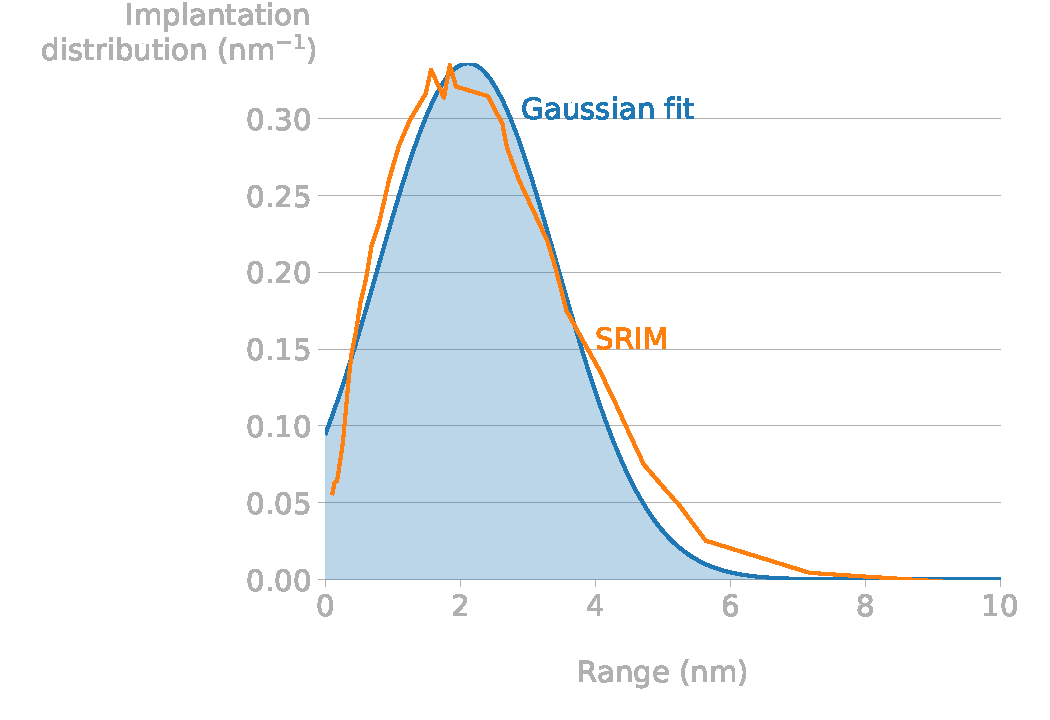
\includegraphics[width=\linewidth]{Figures/Chapter1/srim_implantation_range.pdf}
    \caption{\SI{100}{eV} deuterium implantation profile in tungsten computed from SRIM. Reproduced from \cite{shimada_improved_2019}.}
    \labfig{srim_implantation_profile_example}
\end{figure}

% In order to accurately model this source term, the size of the cells constituing the mesh (the spatial discretisation of the domain) must be less than a nanometre.
% This can be done easily in 1D but is very complicated in higher dimensions, especially when simulating centimetre-sized components.
This volumetric source term can be simplified into a Dirichlet boundary condition (\textit{ie} enforcing the mobile particle concentration at the exposed surface).

Let us consider a volumetric source term of hydrogen $\Gamma = \varphi_\mathrm{imp} \; f(x)$ where $f$ is a narrow Gaussian distribution.
The mobile particles concentration profile can be approximated by a triangular shape \sidecite{schmid_diffusion-trapping_2016} (see Figure \ref{fig:recomb sketch}).

\begin{figure*}[h!]
    \centering
    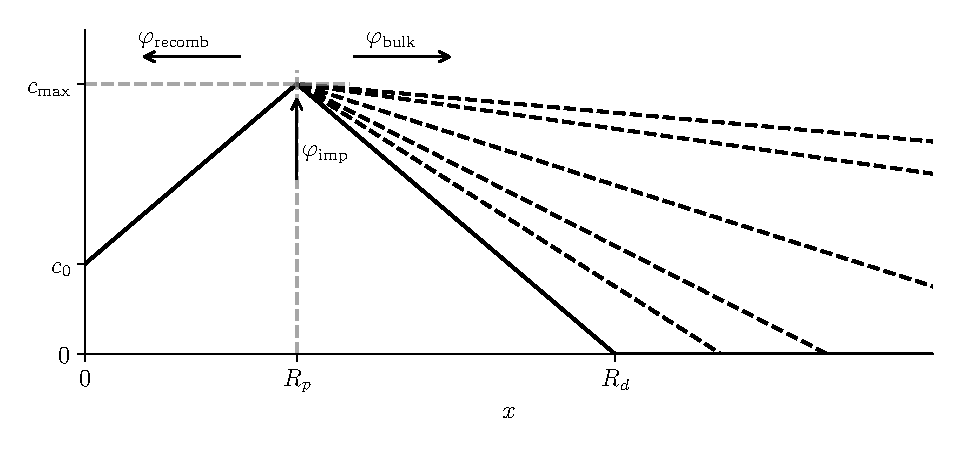
\includegraphics[width=0.75\linewidth]{Figures/Chapter2/recomb_sketch.pdf}
    \caption{Concentration profile with recombination flux and volumetric source term at $x=R_p$. Dashed lines correspond to the time evolution.}
    \label{fig:recomb sketch}
\end{figure*}

The concentration profile is therefore maximum at $x=R_p$.
The expression of $c_\mathrm{max}$ can be obtained by expressing the flux balance at equilibrium:

\begin{equation}
    \varphi_\mathrm{imp} = \varphi_\mathrm{recomb} + \varphi_\mathrm{bulk}
    \label{eq:flux balance}
\end{equation}
where $\varphi_\mathrm{recomb}$ is the recombination flux and $\varphi_\mathrm{bulk}$ is the migration flux.

$\varphi_\mathrm{bulk}$ can be expressed as:
\begin{equation}
    \varphi_\mathrm{bulk} = D \cdot \frac{c_\mathrm{max}}{R_d(t) - R_p}
\end{equation}

% When $t \rightarrow \infty$ or $R_d \gg R_p$ (a ratio of 10 or 100 is enough), $\varphi_\mathrm{bulk} \ll \varphi_\mathrm{recomb}$.
When $R_d \gg R_p$, $\varphi_\mathrm{bulk} \rightarrow 0$.
Equation \ref{eq:flux balance} can therefore be written as:
\begin{equation}
    \varphi_\mathrm{recomb} \approx \varphi_\mathrm{imp}
    \label{eq:flux balance 2}
\end{equation}

Moreover, according to Fick's law, $\varphi_\mathrm{recomb}$ can be expressed as:

\begin{eqnarray}
    \varphi_\mathrm{recomb} &= D \cdot \frac{c_\mathrm{max}-c_{0}}{R_{p}} = \varphi_\mathrm{imp}\\
    \Leftrightarrow c_\mathrm{max} &= \frac{\varphi_\mathrm{imp} R_{p}}{D}+ c_0
    \label{eq:c_max}
\end{eqnarray}

Assuming second order recombination, $\varphi_\mathrm{recomb}$ can also be expressed as a function of the recombination coefficient $K$:

\begin{eqnarray}
    \varphi_\mathrm{recomb} &= K c_{0}^{2} = \varphi_\mathrm{imp}\\
    \Leftrightarrow c_{0} &= \sqrt{\frac{\varphi_\mathrm{imp}}{K}}
    \label{eq:c_0}
\end{eqnarray}

By replacing Equation \ref{eq:c_0} in Equation \ref{eq:c_max} one can obtain:

\begin{equation}
    c_\mathrm{max} = \frac{\varphi_\mathrm{imp} R_{p}}{D}+\sqrt{\frac{\varphi_\mathrm{imp}}{K}}
\end{equation}

As the recombination process becomes fast (\textit{ie} $K \rightarrow \infty$), $c_0 \rightarrow 0$ and $c_\mathrm{max} \rightarrow \frac{\varphi_\mathrm{imp} R_{p}}{D}$.

Since the main driver for the diffusion is the value $c_\mathrm{max}$, when $R_p$ is negligeable compared to the dimension of the simulation domain, one can simply impose this value at the surface.
% This analytical simplification is especially useful to simulate implanted sources near the surface (\textit{eg} plasma implantation) without having to finely discretise the domain to fully represent the gaussian distribution.
% Such a discretisation can be easily done for 1D simulations but is very complex in 2D and 3D and often makes the mesh very large which increases drastically the computational cost.

A transient solution based on trap properties can be derived \sidecite{hodille_study_2016}:
\begin{equation}
    c_\mathrm{max}=\left( \frac{R_p \varphi_\mathrm{imp}}{D} + \sqrt{\frac{\varphi_\mathrm{imp}}{K}} \right) \cdot \frac{\tau}{t} \cdot\left(\sqrt{1+\frac{t}{\tau}}-1\right)^2
\end{equation}
where $\tau$ is a characteristic time expressed by:
\begin{equation}
    \tau = \frac{R_p \sum R_i \, n_i}{8 \varphi_\mathrm{imp}}
\end{equation}
In this expression, $R_i = (p / (k c_\mathrm{max}) + 1)^{-1}$ represents the maximum filling ratio of the trap $i$ and $n_i$ is the trap density.

\subsection{Interface condition: conservation of chemical potential}
% According to Krom \textit{et al} \sidecite{krom_hydrogen_2000}, since the solubility of hydrogen atoms in solids is low, the chemical potential of solute hydrogen $\mu$ is expressed by:
% \begin{equation}
%     \mu = \mu_0 + RT \ln\left( \frac{c_\mathrm{m}}{N_L}\right)
% \end{equation}
% where $\mu_0$ is the chemical potential in a reference state in \si{J.mol^{-1}}, $R$ the ideal gas constant, $T$ the temperature in \si{K}, $c_\mathrm{m}$ the mobile hydrogen concentration in \si{m^{-3}} and $N_L$ the lattice site concentration in \si{m^{-3}}.

% % Assuming that only free hydrogen atoms contribute to the overall flux in the material, the particle flux $J$ in \si{m^{-2}.s^{-1}} can be expressed by Fick's law:
% % \begin{equation}
% %     J = - D \nabla c_\mathrm{m}
% % \end{equation}
% % where $D$ is the diffusion coefficient of hydrogen expressed in \si{m^{2}.s^{-1}}. 


% The local equilibrium at the interface between two materials must ensure  the continuity of both the chemical potential $\mu$ (see Equation \ref{eq: muconservation}) and the particle flux (see Equation \ref{eq: flux conservation}).
% \begin{equation}
%     \mu^- = \mu^+  \label{eq: muconservation}  
% \end{equation}
    
% \begin{equation}
%     D^- \nabla c_\mathrm{m}^- = D^+ \nabla c_\mathrm{m}^+ \label{eq: flux conservation} 
% \end{equation}

The continuity of chemical potential is conveyed by the continuity of $P$, the local partial pressure of hydrogen at equilibrium.
In a metal, $P$ can be expressed from Sievert's law of solubility:
\begin{equation}
    P = (c_\mathrm{m}^-/S^-)^2
\end{equation}
with $S$ the solubility of H in the materials expressed in \si{m^{-3}.Pa^{-0.5}}.
% A way to picture the continuity of chemical potential is to imagine a gas layer at the interface between two materials at a partial pressure $P_\mathrm{eq}$.
% $P_\mathrm{eq}$ can be expressed by the solubility law at the surface of each material.
At the interface between two metallic surfaces, the chemical potential continuity is therefore conveyed by the continuity of the quantity $c_\mathrm{m}/S$.:
\begin{equation}
    (c_\mathrm{m}^-/S^-)^2 = (c_\mathrm{m}^+/S^+)^2
\end{equation}

In the case of a metal in contact with a non-metallic liquid behaving according to Henry's law (\textit{eg} a molten salt):
\begin{equation}
    (c_\mathrm{m}^-/S^-)^2 = c_\mathrm{m}^+/S^+
\end{equation}
with $S$ the solubility of H in the materials expressed in \si{m^{-3}.Pa^{-0.5}} or \si{m^{-3}.Pa^{-1}}.

% This assumption is correct as long as the time needed to reach the equilibrium is low compared to the time of the simulation.
% For long exposure time as well as for high temperatures, the characteristic time is small enough for the equilibrium model to be valid (see page \refpage{Interface transient model}).

% From Equation \ref{eq: c/s conservation}, one can deduce that a solubility discontinuity across an interface induces a discontinuity of mobile hydrogen concentration $c_\mathrm{m}$.
% This can also be interpreted as the chemical potentials at a reference state being different in different materials \sidecite{kirchheim_25_2014}, as the lattice site concentration.

FESTIM ensures the continuity of chemical potential by performing a change of variable in Fick's second law of diffusion with $\phi = c_\mathrm{m}/S$ (in the case of a metal) \sidecite{smith_abaqusstandard_2009} when internal conditions cannot be set.
Neglecting the trapping and generation terms, Equation \ref{eq:mobile} therefore reads:

\begin{align}
    \frac{\partial \phi S}{\partial t} &= \nabla \cdot\left(D \nabla \phi S\right) + f \nonumber \\
    &=\nabla \cdot\left( D S \nabla \phi + D \phi \nabla S\right) + f \label{eq: diffusion equation changed}
\end{align}

% Because $\phi$ is computed, the ratio $c_\mathrm{m}/S$ is continuous by default at the material interfaces.

% This second approach is used for instance in the \textit{mass-diffusion} procedure of the Abaqus code \sidecite{smith_abaqusstandard_2009}.
% This interface model has also been implemented into the current hydrogen transport code FESTIM \sidecite{delaporte-mathurin_finite_2019} using FEniCS \sidecite{alnaes_fenics_2015}.

After solving Equation \ref{eq: diffusion equation changed} for $\phi$, $c_m$ can be retrieved by multiplying the solution by $S$.

\section{Heat transfer}
Due to the numerous processes that are thermally activated, it is essential to have an accurate temperature field.
Moreover, most tokamak plasma facing components are exposed to intense heat fluxes and are actively cooled, exhibiting high temperature gradients.
The temperature fields are even more complex when dealing with non-trivial geometries like monoblocks or breeding blankets.
For these reasons, heat transfers need to be modelled.

The equation describing heat conduction in solids is described as follows:
\begin{equation}
    \rho \cdot C_p \frac{\partial T}{\partial t}=\nabla \cdot (\lambda \nabla T)
    \label{eq:heat equation}
\end{equation}
where $\rho$ is the density of the material in \si{kg.m^{-3}}, $C_p$ its specific heat capacity expressed in \si{J.kg^{-1}.K^{-1}} and $\lambda$ the thermal conductivity expressed in \si{W.m^{-1}.K^{-1}}.

The thermal properties $C_p$, $\rho$ and $\lambda$ are usually temperature dependent.

For heat transfer problems, three types of boundary conditions can be imposed.

First, the temperature can be fixed on the boundary with a Dirichlet boundary condition (see Equation \ref{eq:dirichlet bc T}).
\begin{equation}
    T = T(x, y, z, t) \quad \text { on } \partial \Omega
    \label{eq:dirichlet bc T}
\end{equation}
where $\partial \Omega$ is the domain boundary.

On the other hand, a heat flux can also be imposed by enforcing the temperature gradient (see Equation \ref{eq: neumann bc T}).
This condition is called a Neumann condition.
\begin{equation}
    -\lambda \nabla T \cdot \mathbf{n} = f(x, y, z, t) \quad \text { on } \partial \Omega
    \label{eq: neumann bc T}
\end{equation}
where $\lambda$ is the thermal conductivity in \si{W.m^{-1}.K^{-1}}, $\mathbf{n}$ is the boundary normal vector and $\partial \Omega$ is the domain boundary.

Finally, to model a convective heat flux when the surface is in contact with a fluid (\textit{eg} cooling pipes, natural convection...), a Robin boundary condition needs to be employed (see Equation \ref{eq: convective bc T}).
\begin{equation}
    -\lambda \nabla T \cdot \mathbf{n} = h (T - T_\mathrm{ext}) \quad \text { on } \partial \Omega
    \label{eq: convective bc T}
\end{equation}
where $\lambda$ is the thermal conductivity in \si{W.m^{-1}.K^{-1}}, $\mathbf{n}$ is the boundary normal vector, $h$ is the heat transfer coefficient in \si{W.m^{-2}.K^{-1}}, $T_\mathrm{ext}$ is the fluid temperature in \si{K} and $\partial \Omega$ is the domain boundary.
The heat transfer coefficient can be dependent on the temperature and the flow characteristics.
It is obtained by computing the Nusselt number from correlations linking it to the Reynolds number of the flow and the Prandtl number of the fluid \sidecite{poirier_correlations_2016} (\textit{eg} Dittus-Boetler, Sieder-State, Gnielinski, ...).
Once the Nusselt number is known, the heat transfer coefficient $h$ reads:
\begin{equation}
    h = \frac{\lambda \, \textit{Nu}}{L}
\end{equation}
with $\lambda$ the thermal conductivity of the fluid in \si{W.m^{-1}.K^{-1}}, $\textit{Nu}$ the Nusselt number and $L$ the characteristic length in \si{m}.


\section{Implementation}


The models described in this Section can be hard to solve analytically for complex problems (complex geometries, transients, combined boundary conditions, etc).
The code FESTIM \sidecite{delaporte-mathurin_finite_2019} was therefore developped in order to solve these equations numerically.

\subsection{The finite element method: FEniCS}
FESTIM is based on the Finite Element Method to solve this set of differential equations and boundary conditions.
Several finite element libraries are available open-source (deal.II \sidecite{arndt_dealii_2021}, MFEM \sidecite{kolev_tzanio_modular_2010}, MOOSE \sidecite{permann_moose_2020}, FreeFEM++ \sidecite{hecht_new_2012}, ...).
The open-source python/C++ package FEniCS \sidecite{alnaes_fenics_2015} was employed.
The finite element method is a versatile tool that can solve any partial differential equation on an arbitrary geometry in 1D, 2D or 3D.
The main advantage of this method compared to the finite difference method is the simplicity of its application to complex geometries and unstructured meshes.
Indeed, implementing a finite difference scheme for such a problem would be tedious and extra care must be taken for mistakes in the implementation could result in losses in efficiency and accuracy of the numerical solution.

This section will illustrate the finite element method applied to a simple diffusion equation (see Equation \ref{eq: example poisson}).

\begin{align}
    -\nabla^2 u &= f \\
    u &= 0 \quad \text{on    } \delta \Omega
    \label{eq: example poisson}
\end{align}

The first step of the finite element method is to represent the solution $u$ as a combination of piecewise polynomials (see Equation \ref{eq: FEM solution}).

\begin{equation}
    u = \sum^N_{i=0}u_i \phi_i(x, y, z)
    \label{eq: FEM solution}
\end{equation}
where $N$ is the number of degrees of freedom, $u_i$ are the coefficient to be determined (called degrees of freedom) and $\phi_i$ are polynomials (see Figure \ref{fig: example approximated solution}).

\begin{figure}
    \centering
    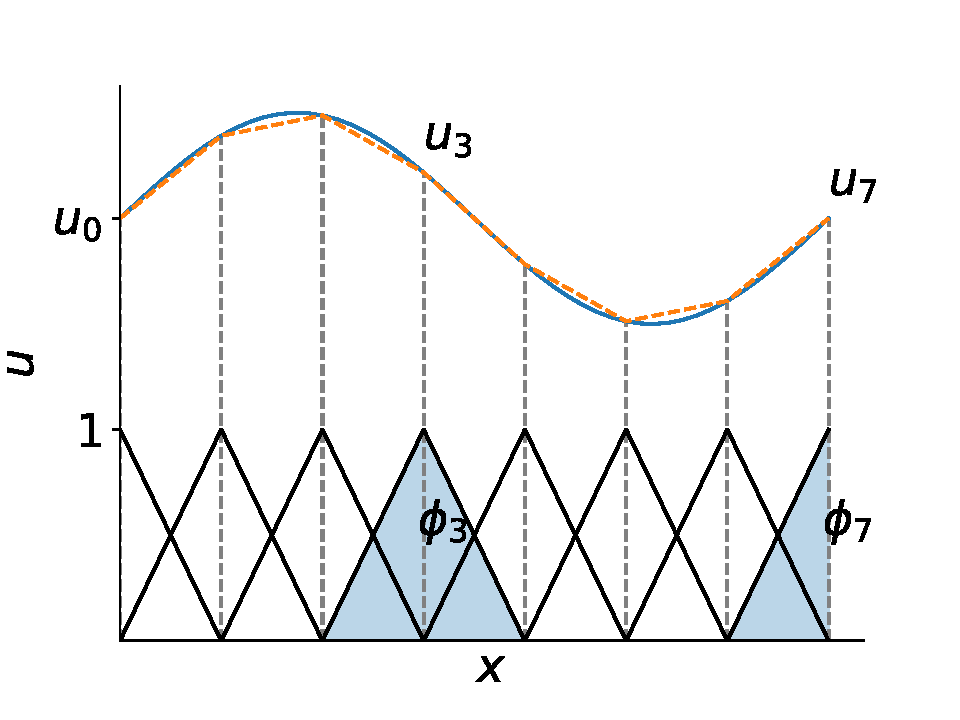
\includegraphics[width=\linewidth]{Figures/Chapter2/approximated_solution.pdf}
    \caption{1D example of an approximated solution $u$ (exact in blue, approximated in orange) with basis functions $\phi_i$}
    \label{fig: example approximated solution}
\end{figure}


The second step is to build a variational formulation (also called \textit{weak form}) of the governing equation \ref{eq: example poisson}.
To do so, the "recipe" is to multiply the PDE by a function $v$ (called the \textit{test function}) and integrate over an arbitrary element $\Omega_e$.
The following expression is obtained:
\begin{equation}
    \int_{\Omega_e} -\nabla^2 u v dx = \int_{\Omega_e} f v dx \quad \forall v
    \label{eq: weak form 1}
\end{equation}

When using $N+1$ different test functions, Equation \ref{eq: weak form 1} then gives rise to a system of $N+1$ equations.
This form is called the weak form because it relaxes the requirement of Equation \ref{eq: example poisson} and instead requires to solve Equation \ref{eq: weak form 1} for all test functions.

Equation \ref{eq: weak form 1} needs now to be rewritten in order to only have first order derivatives.
To do so, Gauss-Green's lemma is employed:
\begin{equation}
    \int_{\Omega_e} -\nabla^2 u v dx = \int_{\Omega_e} \nabla u \cdot \nabla v dx - \int_{\partial \Omega_e} \frac{\partial u}{\partial n} v dx
    \label{eq: gauss-green}
\end{equation}

The variational form therefore reads:
\begin{equation}
    \int_{\Omega_e} \nabla u \cdot \nabla v dx = \int_{\Omega_e} f v dx + \int_{\partial \Omega_e} \frac{\partial u}{\partial n} v dx \quad \forall v
    \label{eq: weak form 2}
\end{equation}
where the last term of the equation either vanishes due to Dirichlet boundary conditions (or is imposed).

From Equation \ref{eq: weak form 2}, a system of $N+1$ equations can be solved to determine the coefficients $u_i$ in Equation \ref{eq: FEM solution}.
Once the $u_i$ coefficients are known, an approximated solution can be computed.

\subsection{Main features of FESTIM}
FESTIM provides an even higher level of abstraction than FEniCS by providing a user-friendly interface dedicated to H transport and H transfer problems.
Users only have to provide inputs such as material properties, traps properties, geometry, solving parameters, without having to dive into the finite element implementation.

% user friendly
Multi-dimensional transient simulations coupled with heat transfer can therefore be run fairly easily without finite element knowledge.
Nevertheless, since FESTIM is object-oriented, advanced users will always be able to turn FESTIM inside-out to adapt the code to their specific needs (specific boundary conditions, slight changes in the governing equations...).
Since FESTIM is written in python - which is a fairly easy-to-learn programming langage - no advanced level of coding is required.

% physics
As mentioned above, FESTIM simulates the transport (diffusion and trapping) of H and additional physics can be incorporated, such as the Soret effect (also called heat of transport) and conservation of chemical potential at interfaces...
Various types of boundary conditions are available for both the H transport (imposed concentration, recombination flux, dissociation flux, implanted source approximation...) and the heat transfer problems (imposed temperature, imposed flux, convective flux...).
Traps densities in FESTIM can also be time-dependent allowing the users to simulate extrinsic traps (\textit{eg} irradiation induced traps, stress induced traps...).

% geometry
Thanks to the finite element method, geometries used in FESTIM can be complex (see Figure \ref{fig: example mesh}).
The meshing capability of FESTIM is limited to 1D meshes and it was decided to instead make FESTIM accept (with the XDMF format) complex meshes from third-party applications dedicated to meshing such as SALOME or GMSH.
These third-party applications can for instance be usefull to run CAD-based simulations.
Users can also decide to use the FEniCS built-in meshing tool.

\begin{figure}
    \centering
    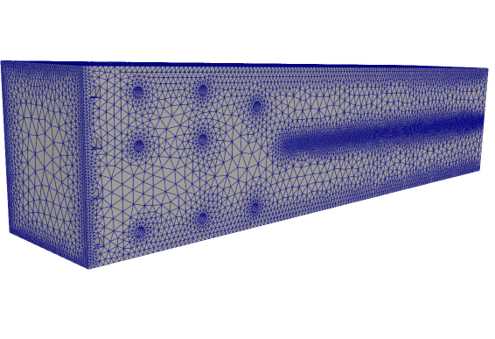
\includegraphics[width=0.5\linewidth]{Figures/Chapter2/example_mesh.png}
    \caption{Example of a complex 3D geometry (here a breeding blanket section) mesh readable by FESTIM \cite{dark_influence_2021}.}
    \label{fig: example mesh}
\end{figure}

% visualisation
Similarly, FESTIM (FEniCS) visualisation functions are limited.
FESTIM is not a graphical application but the files generated by FESTIM (XDMF, CSV, TXT) can easily be read and post-processed by specialised tools such as Paraview \sidecite{ahrens_paraview_2005}, matplotlib \sidecite{hunter_matplotlib_2007}, NumPy \sidecite{harris_array_2020}, etc.

% what FE
Regarding the default finite elements used in FESTIM are Continuous Galerkin elements but it can be switched to Discontinuous Galerkin when needed.
This is usefull when the trapped concentration is discontinuous and help avoiding under- or over-shoots in the concentration field.

% Adaptive step size
When dealing with transient problems, FESTIM provides an adaptive stepsize allowing the stepsize to increase (by a user-defined factor) when the convergence criterion is easily reached by the solver.
This greatly improve the performance of the code since less timesteps are needed.



\section{Verification \& Validation}

Before using the FESTIM code for analysis, it has to be verified and validated.
The verification \& validation process (often called V\&V) has two goals: (1) to prove that the governing equations are correctly solved and that the code is error free and (2) to demonstrate that the governing equations actually reproduce processes observed experimentally.
In other words, verification is answering the question "Are we building the code right?" and validation is answering the question "Are we building the right code?".

This Section details the V\&V of the FESTIM code.

\subsection{Analytical verification}
Verification is the process of ensuring the governing equations are correctly solved in FESTIM.
This is an integral part of every simulation code for it guarantees the code is error free.
It is generally hard to simply substitute this process by code comparison (cross-checks between two different codes) because often the codes are implemented differently.
Moreover, if the code we are comparing with is not verified, then obtaining similar results does not give any guarantee on the code accuracy as two different codes can have the same bug.

Several methods can be used to verify a code but the \gls{mes} and the \gls{mms} are employed here.

Both methods consist in comparing a computed solution with an exact solution and measuring the error.
The exact solution in the \gls{mes} is obtained by solving the governing equations analytically.
When using the \gls{mms}, the problem is reversed: an arbitrary exact solution (called \textit{manufactured solution}) is chosen and injected in the governing equations.
It is then possible to determine source terms and boundary conditions.
These are then fed into the code and the computed solution is compared to the manufactured (exact) solution.

This \gls{mms} is often used to unravel the complexity of governing equations \sidecite{dudson_verification_2016, roache_code_2002}.
This is particularly useful when dealing with complex geometries or to exercise non-trivial material properties.

This section describes two verification cases of \gls{festim}.
The first one uses the \gls{mes} and the second one the \gls{mms}.
More complex and thorough verification cases are shown in Appendix \ref{appendix verification}.

\subsubsection{Case 1: H transport (\gls{mes})} \labsec{analytical}

\begin{figure}
    \centering
    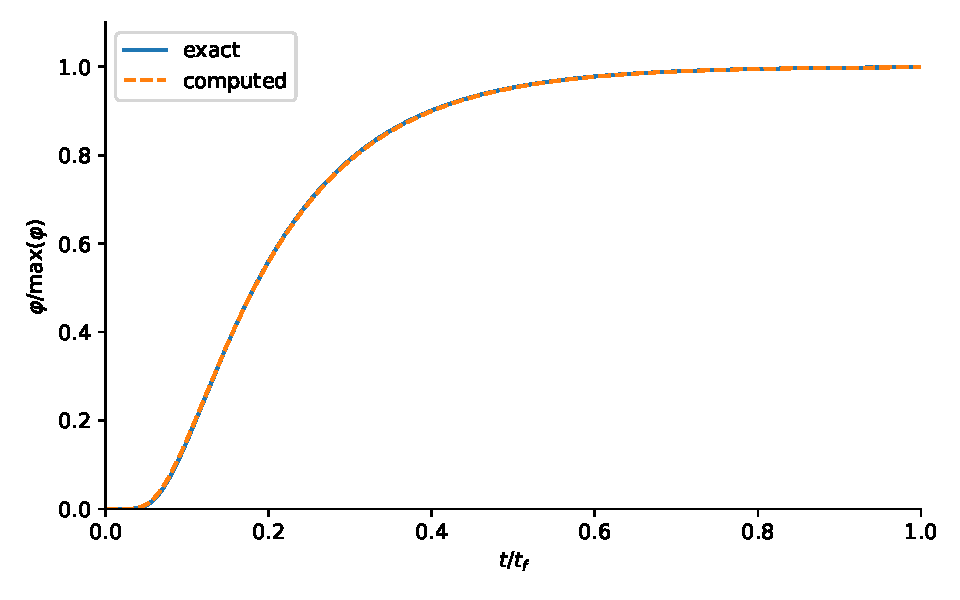
\includegraphics[width=\linewidth]{Figures/Chapter3/mes_festim_effective_diffusion.pdf}
    \caption{Temporal evolution of the outward particle flux $\varphi$ at $x=l$ (Case 1).}
    \labfig{FESTIM vs analytical}
\end{figure}

% Although validation against experiments could show that FESTIM is able reproduce the data with a given set of parameters, objective verification against analytical solutions is first required to ensure that the governing \refeq{mobile} and \refeq{trapped} are solved correctly.

For this verification case, a 1D slab is considered with a thickness $l$.
The concentration of mobile particles was set to $c_0$ on one side of the slab and set to zero on the other side.
Only one trap is considered in this case and its density $n$ is homogeneously distributed.

The trapping parameter $\zeta$ is defined in \sidecite{longhurst_verification_2005} as follows:
\begin{equation}
    \zeta = \frac{p}{k \: n} + \frac{c_\mathrm{m}}{n}
\end{equation}

In our case, we choose the trapping and detrapping rates $k$ and $p$, the concentration $c_0$ and the temperature $T$ so that $\zeta \gg \frac{c_\mathrm{m}}{n}$.
This condition is equivalent to having the trap filling ratio $(p / (k \, c_\mathrm{m}) + 1)^{-1} \ll 1$.
This is known as the \textit{effective diffusivity regime} where the diffusion is almost identical to the case where there are no traps.
In this regime, the governing equations are identical as a pure diffusion regime and are therefore easy to solve analytically.

The coefficient $D$ is then replaced by an effective diffusion coefficient:
\begin{equation}
    D_\mathrm{eff} = \frac{D}{1+\frac{1}{\zeta}}
\end{equation}
The particle flux at the background surface ($x=l$) is expressed in $\si{H.m^{-2}.s^{-1}}$ and finally defined in \cite{longhurst_verification_2005} by:
\begin{equation}
    \varphi(t) = \frac{c_0 D}{l}\bigg[1+2\sum_{m=1}^{\infty}(-1)^m \exp\bigg(-m^2\frac{\pi^2 \:D_\mathrm{eff} \: t}{l^2}\bigg)\bigg]
\labeq{flux analytical}
\end{equation}
In \refeq{flux analytical}, the infinite sum has been truncated at $m=10000$.

All the parameters used in this verification case are defined in \reftab{parameters analytical verification}.
These parameters have been chosen for the sake of verification and do not necessarily represent realistic conditions as verification is a mathematical exercise.
\begin{table}
    \centering
    \begin{tabular}{p{2.3cm} p{2cm} r}
        Parameter & Units & Value \\
        \hline
        \\
        $D_0$ & $\si{m^2.s^{-1}}$ & 2.0 \\
        $k_0$ & $\si{m^3.s^{-1}}$ & 0.01 \\
        $p_0$ & $\si{s^{-1}}$ & 1.0 \\
        \\
        $E_D$ & $\si{eV}$ & 0.2 \\
        $E_k$ & $\si{eV}$ & 0.1 \\
        $E_p$ & $\si{eV}$ & 0.1 \\
        \\
        $c_0$ & $\si{m^{-3}}$ & 2.0 \\
        $n$ & $\si{m^{-3}}$ & 2.0 \\
        $l$ & $\si{m}$ & 1.5\\
        \\
        $T$ & $\si{K}$ & 300 \\
        \\
        $t_f$ & $\si{s}$ & 2000 \\
        \\
    \end{tabular}
    \caption{Parameters used for the analytical verification (Case 1).}
    \labtab{parameters analytical verification}
\end{table}
One can notice on \reffig{FESTIM vs analytical} that the numerical results are in good agreement with the analytical solution.
The relative L2 error between analytical and numerical solutions was found to be $\approx 1 \%$ with 1000 piecewise linear elements (\gls{p1}) and a stepsize of \SI{1}{s}.
This value decreases with the stepsize and with the element size (see \reffig{MES evolution of L2 error as function of dt and dx}).
\begin{figure}
    \centering
    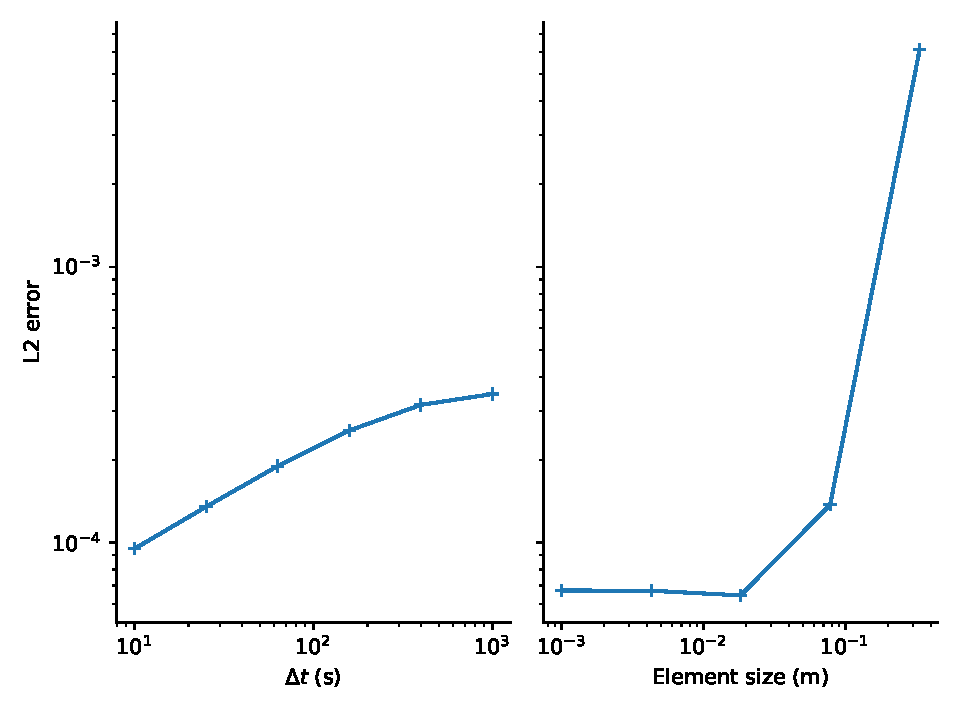
\includegraphics[width=\linewidth]{Figures/Chapter2/error_vs_element_size_and_dt.pdf}
    \caption{Evolution of the L2 error on $\varphi$ as a function of the stepsize and element length (Case 1).}
    \labfig{MES evolution of L2 error as function of dt and dx}
\end{figure}


Since this test case is very similar to a pure diffusion case, it does not exercise all terms of the governing equations.
To do so, the governing equations would have to be solved for a generic case which proves to be complex.
This is why the \gls{mms} will be used instead.

\subsubsection{Case 2: H transport (\gls{mms})} \labsec{mms}

\paragraph{Principle}
The \gls{mms} is often used to unravel the complexity of governing equations \sidecite{dudson_verification_2016, roache_code_2002}.
This is particularly useful when dealing with complex geometries or to exercise non-trivial material properties.

The principle of the \gls{mms} is to manufacture an exact solution.
Again, physical realism is not a concern here as verification is a mathematical exercise.
This manufactured solution needs to be non-trivial in order to test the robustness of the implementation.
It is then passed through the governing equations (either the heat equation or the hydrogen transport equations) and source terms are obtained.

Let us take a simple example with the Poisson equation defined on a 1D domain $[x_1, x_2]$:
\begin{equation}
    \frac{\partial u}{\partial t} = \frac{\partial^2 u}{\partial x^2} + q
    \labeq{poisson eq demo mms}
\end{equation}
where $u$ is the unknown, $q$ is the source term.

The manufactured solution is arbitrarily defined as:
\begin{equation}
    U(t, x) = A + \sin{(x + B t)}
\end{equation}
where $A$ and $B$ are real numbers, $t$ is the time, and $x$ is the spatial coordinate.
By replacing $u$ by $U(t, x)$ in \refeq{poisson eq demo mms}, we can identify the source term $q$ that would produce the solution $U(t, x)$:

\begin{equation}
    Q(t, x) = B \cos{(x + B t)} + \sin{(x + B t)}
\end{equation}

Several boundary conditions can be used to produce $U(t, x)$.
We can for instance set a Dirichlet boundary condition on the boundaries $x=x_1$ and $x=x_2$:
\begin{align}
    u(t, x_1) &= U(t, x_1) \\
    u(t, x_2) &= U(t, x_2)
\end{align}

or Neumann boundary conditions:
\begin{align}
    \frac{\partial u(t, x)}{\partial x}\Big | _{ x=x_1} &= \frac{\partial U(t, x)}{\partial x} \Big | _{ x=x_1} \\
    \frac{\partial u(t, x)}{\partial x}\Big | _{ x=x_2} &= \frac{\partial U(t, x)}{\partial x} \Big | _{ x=x_2}
\end{align}

or even a combination of Dirichlet and Neumann boundary conditions.

By solving \refeq{poisson eq demo mms} with $q = Q(t, x)$ and initial condition $u = U(0, x)$, we can obtain the computed solution $u_\mathrm{computed}$.
The error between the computed solution $u_\mathrm{computed}$ and the exact solution $U(t, x)$ can be calculated to assess the code accuracy.

\paragraph{Case 2a: Application to 1D hydrogen transport}

Let us apply the \gls{mms} to the hydrogen transport model on a 1D domain $\Omega$.
In order to exercise all terms in \refeq{mobile} and \refeq{trapped}, the following manufactured solutions are chosen:
\begin{equation}
    \begin{cases}
    c_{m_D} = 1 + x^2 + \sin(t) \\
    c_{{t,1}_D} = 1 + x^2 + \cos(t)
    \end{cases}
    \labeq{manufactured solutions}
\end{equation}

By combining \refeq{mobile}, \refeq{trapped} and \refeq{manufactured solutions}, one can obtain the following source terms:
\begin{equation}
    \begin{cases}
    f = \cos(t) - \sin(t) - 2D \\
    g_1 = p_1 c_{{t,1}_D} - k_1 c_{m_D} ( n_1 - c_{{t,1}_D}) - \sin(t)
    \end{cases}
    \labeq{sources}
\end{equation}
$f$ is the source term of the mobile concentration equation and $g_1$ is the source term of the trapped concentration equation.

where $g_1$ is an additional source term in \refeq{trapped}.
The Dirichlet boundary conditions for $c_\mathrm{m}$ and $c_{t,1}$ are:

\begin{equation}
    \begin{cases}
    c_\mathrm{m} = 1 + x^2 + \sin(t) \quad \text{on } \partial \Omega \\
    c_{t,1} = 1 + x^2 + \cos(t) \quad \text{on } \partial \Omega 
    \end{cases}
\end{equation}
where $\partial\Omega$ is the boundary of the domain.
Finally, initial values for $c_\mathrm{m}$ and $c_{t,i}$ are:
\begin{equation}
    \begin{cases}
    c_\mathrm{m}(t=0) = 1 + x^2 \\
    c_{t,1}(t=0) = 2 + x^2
    \end{cases}
\end{equation}
Once all these parameters are fed into FESTIM, one can easily compare the computed solution with the exact solution in \refeq{manufactured solutions}.
The L2-norm $E_{c_\mathrm{m}}$ can then be calculated as follows:
\begin{equation}
    E_{c_\mathrm{m}} = \sqrt{\int_\Omega(c_{m_D} - c_\mathrm{m})^2dx}
\end{equation}
The evolution of $E_{c_\mathrm{m}}$ as function of the element size $h$ is shown on \reffig{error vs h}.
One can notice that $E_{c_\mathrm{m}}$ increases as $A\cdot h^k$.
This is known as the \textit{asymptotic regime} and the coefficient $k$ is called the convergence rate.
$k$ typically approaches $N+1$ as $h$ approaches zero, $N$ being the order of the finite elements.
In this case, $k \approx 2$ as expected since first order finite elements have been used.

\begin{figure}
    \centering
    \includegraphics[width=1\linewidth]{"Figures/Chapter3/L2 error on Cm vs h"}
    \caption{Evolution of the L2 norm of the error as function of element size h for the 1D H transport case (Case 2a).}
    \labfig{error vs h}
\end{figure}

\paragraph{Case 2b: Application to 2D hydrogen transport}


The same method can be applied to a 2D case.
Let us choose the following steady state test problem on a domain $\Omega = [0, 1] \times [0, 1]$ with the manufactured solution $c_D(x, y) = \sin(\omega \pi x) \sin(\omega \pi y)$.

\begin{align}
    \nabla \cdot D \nabla c_\mathrm{m} &= -f_1 \\
    k c_\mathrm{m} (n - c_\mathrm{t}) - p c_\mathrm{t} &= -f_2 \\
    c_\mathrm{m} &= c_\mathrm{t} = c_D \text{  on  } \partial \Omega \\
    D &= 2 \\
    p &= 3 \\
    k &= 2 \\
\end{align}

The source terms $f_1$ and $f_2$ and the boundary conditions can be obtained in a similar fashion by replacing $c_\mathrm{m}$ and $c_\mathrm{t}$ in the governing equations.

It was shown that the computed solutions was similar to the exact solutions (see \reffig{results MMS 2D H transport}).
Moreover, the convergence rates confirm the mesh dependency of the computed solutions' accuracy (see \reffig{convergence rates H}).
% A super-convergence is observed for the P2 elements.

\begin{figure*}
    \centering
    \begin{subfigure}{0.3\linewidth}
        \centering
        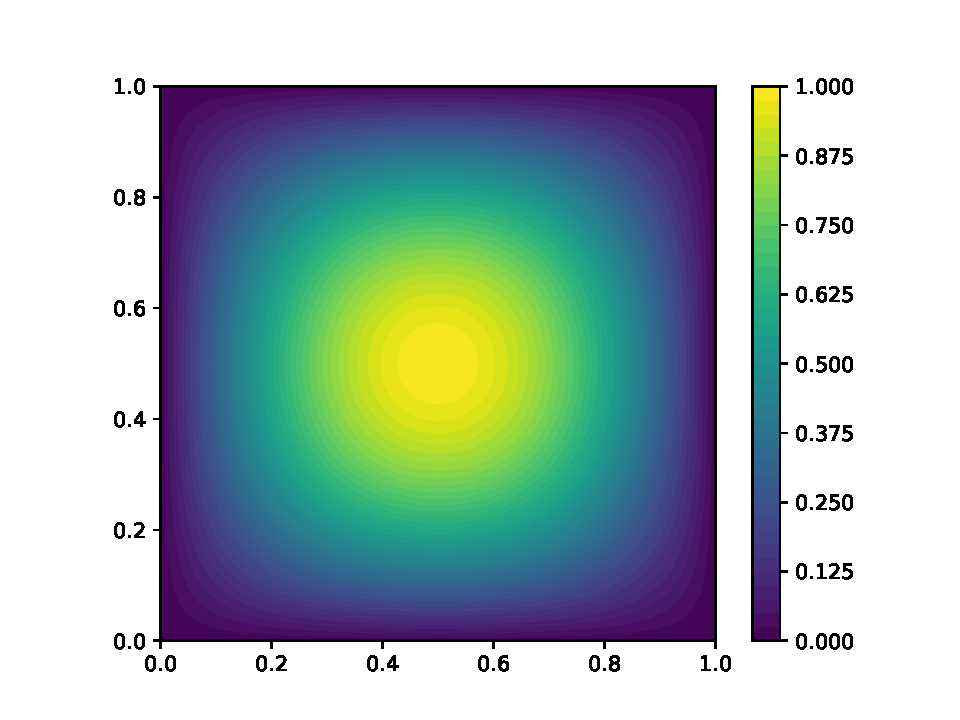
\includegraphics[width=\linewidth]{Figures/Chapter2/c_m.pdf}
        \caption{Computed $c_\mathrm{m}$ (64 elements).}
    \end{subfigure}%
    \begin{subfigure}{0.3\linewidth}
        \centering
        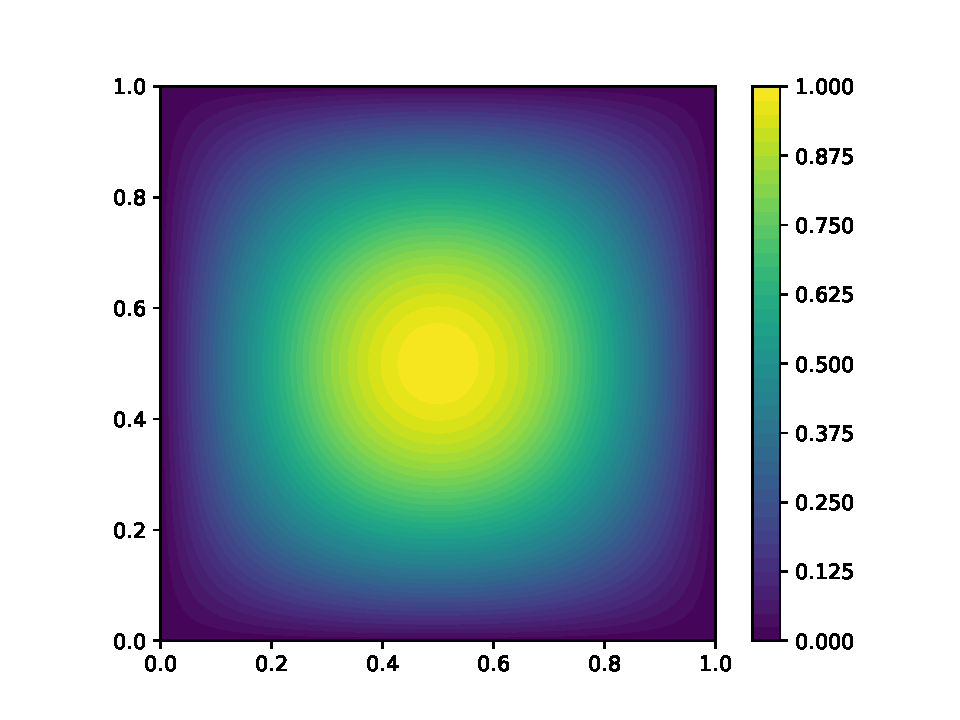
\includegraphics[width=\linewidth]{Figures/Chapter2/c_t.pdf}
        \caption{Computed $c_\mathrm{t}$ (64 elements).}
    \end{subfigure}%
    \begin{subfigure}{0.3\linewidth}
        \centering
        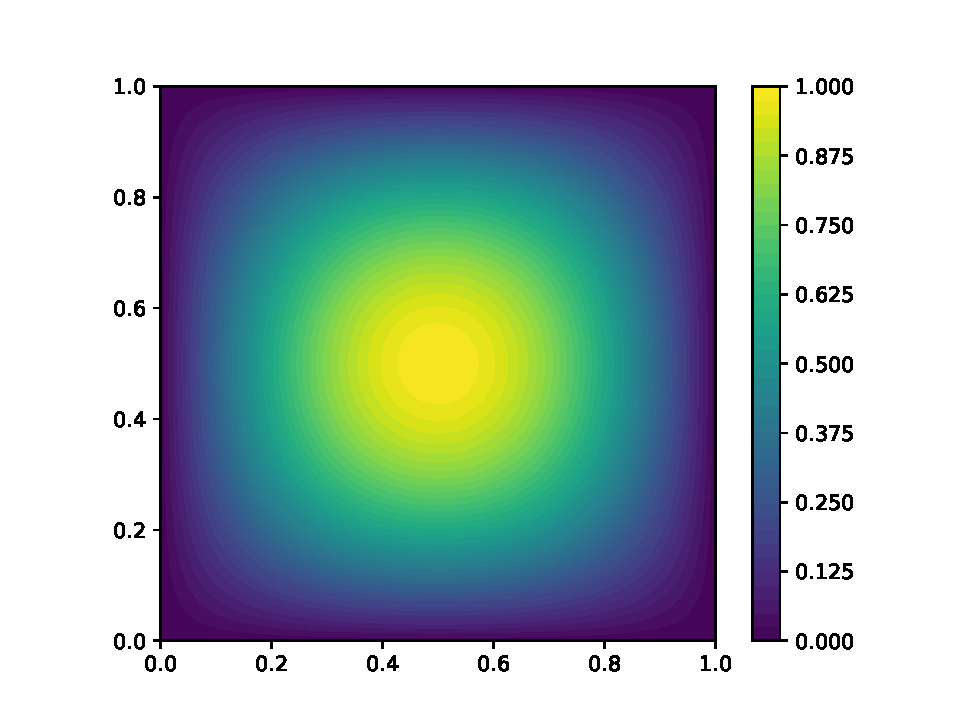
\includegraphics[width=\linewidth]{Figures/Chapter2/c_exact.pdf}
        \caption{Exact solution $c_D$.}
    \end{subfigure}
    \caption{Comparison of the computed concentrations with the exact solution (Case 2b).}
    \labfig{results MMS 2D H transport}
\end{figure*}

\begin{figure}
    \centering
    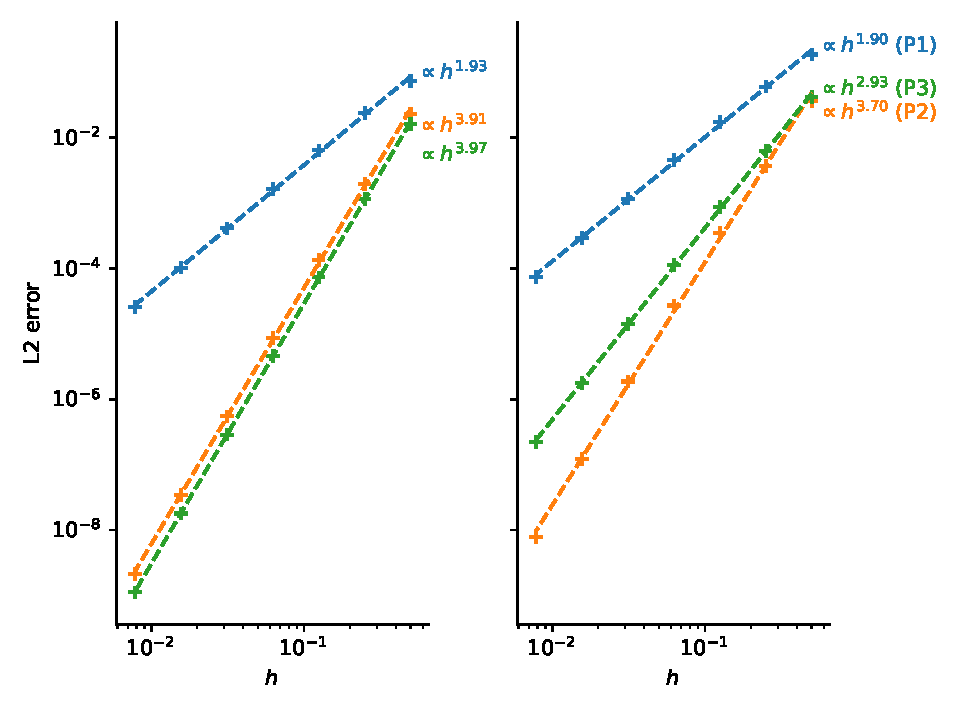
\includegraphics[width=\linewidth]{Figures/Chapter2/convergence_rate_H.pdf}
    \caption{Evolution of the L2 error on $c_\mathrm{m}$ (left) and $c_\mathrm{t}$ (right) showing the convergence rates for the 2D H transport case (Case 2b).}
    \labfig{convergence rates H}
\end{figure}



\subsection{Experimental validation}

Now that the code has been verified (\textit{ie} solves the governing equations correctly), experimental validation is still required to check that these equations actually represent real life processes.
A very good example of real life experiments that can be reproduced are Thermo-Desorption Spectroscopy (TDS) experiments also called Thermally Programmed Desorption (TPD) experiments.
The principle of such experiments is to load small samples with H isotopes (H, D, or T) - either with a gas infusion or via plasma implantation - and heat them up to different temperatures to desorb the trapped H.
By measuring the outgassing flux of particles throughout the time of the experiment, desorption spectra are obtained.
These spectra often exhibit several peaks and each peak correspond to a kind of trap.

This technique is therefore employed to characterise materials and determine their defects. 
It is also a very good application case for experimental validation of the H transport model.

This section describes the technique that was employed to easily reproduce these TDS experiments.
% Several application cases will also be shown on W, Al, EUROFER, and Be.

\subsubsection{Methodology} \label{methodology}
Fitting experimental data by manually tweaking parameters as in \sidecite{yu_deuterium_2019, hodille_macroscopic_2015} can be really time-consuming, sometimes days in some cases.
Moreover, some possible solutions in the parameter space might be missed by the user.
This process has been automated by embedding \gls{festim} in a minimisation algorithm.

As in manual fitting, the parametric optimisation problem is solved by minimising a function representing the residual between simulated results and some reference data.
This function $f$ is called \textit{cost function}.
Considering fitting one or several \gls{tds} spectra (in order to identify for instance trapping parameters or diffusion coefficients), $f$ can simply be the mean absolute error described in Equation \ref{eq:cost function} representing the residual between the simulated spectrum and the experimental reference: 

\begin{equation}
    f(\textbf{x})=\frac{\sum_{i=0}^{N}  \alpha_i(T_i)\left| d_{i}-d_{\mathrm{sim}}\right|}{\sum_{i=0}^{N}  \alpha_i(T_i)}
    \label{eq:cost function}
\end{equation}

where \textbf{x} is the set of parameters used for the simulation, $d_\mathrm{sim}$ are the values of the simulated spectrum, $N$ is the number of experimental points $(T_i, d_i)$.
In Equation \ref{eq:cost function}, $f(\textbf{x})$ can be weighted by coefficients $\alpha_i$ in order to have a better fit on specific regions of the spectrum.
%Note that this cost function could as well be a root mean square error or any type of residual.

The parametric optimisation problem can now be solved by finding the minimum of the cost function $f$.
The global optimisation routine is illustrated on Figure \ref{fig:diagramm}.
\begin{figure}
    \centering
    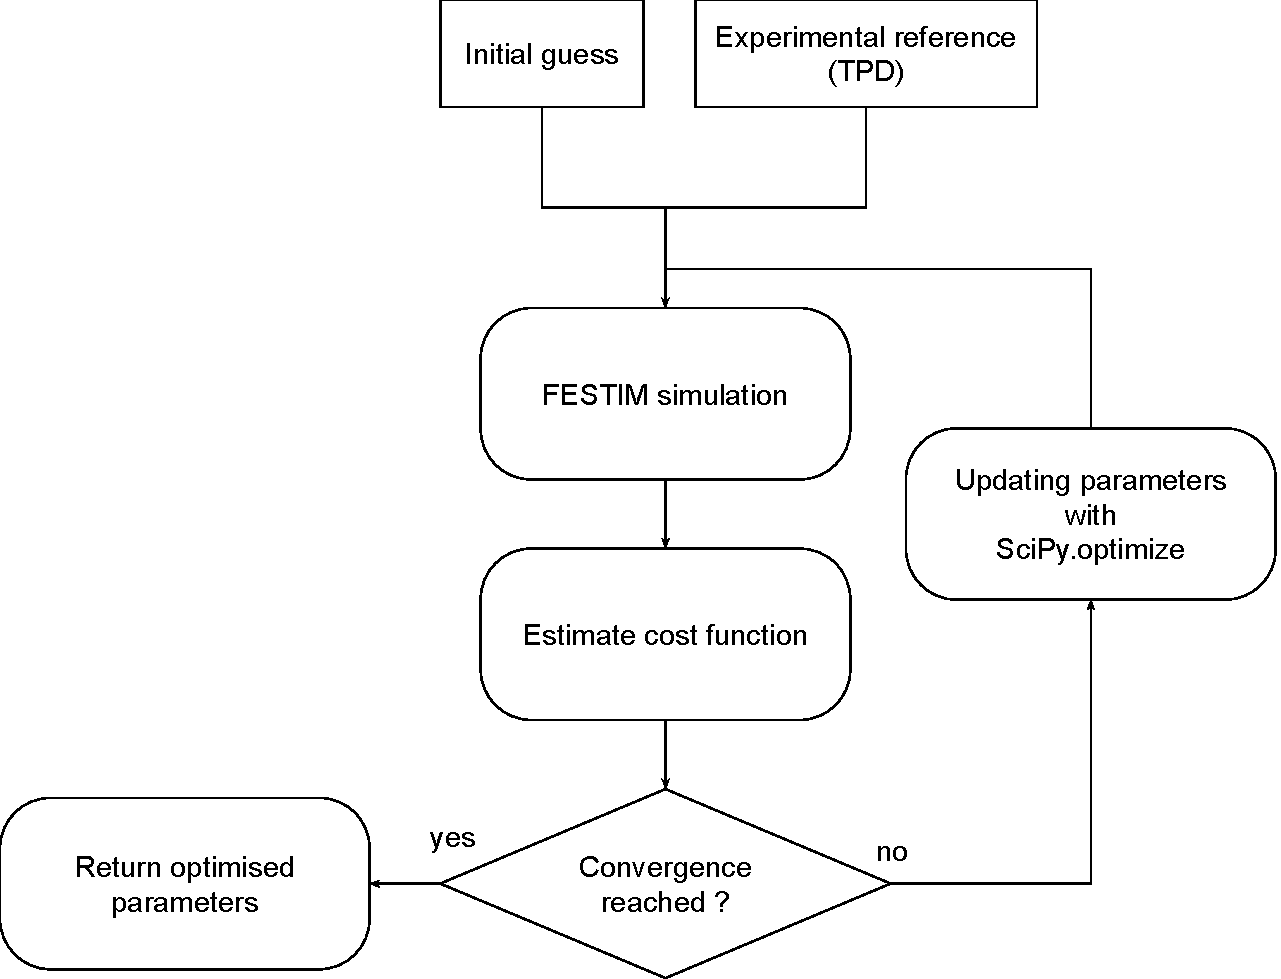
\includegraphics[width=\linewidth]{Figures/Chapter3/Parametric_optimisation/algorithm diagram.pdf}
    \caption{Diagram of the embedding of FESTIM within a parametric optimisation routine based on SciPy \cite{virtanen_scipy_2020}.}
    \label{fig:diagramm}
\end{figure}

A comparative study of the several optimisation algorithms which can be employed has been made.
These algorithms require the user to give an initial set of parameters called \textit{initial guess} and evaluate the cost function with several parameters sets until the convergence criterion is reached.
As in \sidecite{drexler_model-based_2019}, the Python package SciPy \sidecite{virtanen_scipy_2020} will be employed.

Four minimisation algorithms have been benchmarked against a test case.
In the following example an experimental \gls{tds} spectrum from Ogorodnikova et al.\ \sidecite{ogorodnikova_deuterium_2003} will be fitted and materials properties such as trap density and detrapping energy will be identified.
For this example case, two intrinsic traps and one extrinsic trap are set.
The only free parameters are $E_1$ and $n_1$, respectively the detrapping energy and density of trap 1.
The other parameters are constrained and described in \sidecite{delaporte-mathurin_finite_2019}.
The cost function $f$ has been plotted on Figure \ref{fig:cost function} as function of $E_1$ and $n_1$.

\begin{figure*} [h!]
    \centering
        \begin{subfigure}[t]{0.7\linewidth}
            \centering
            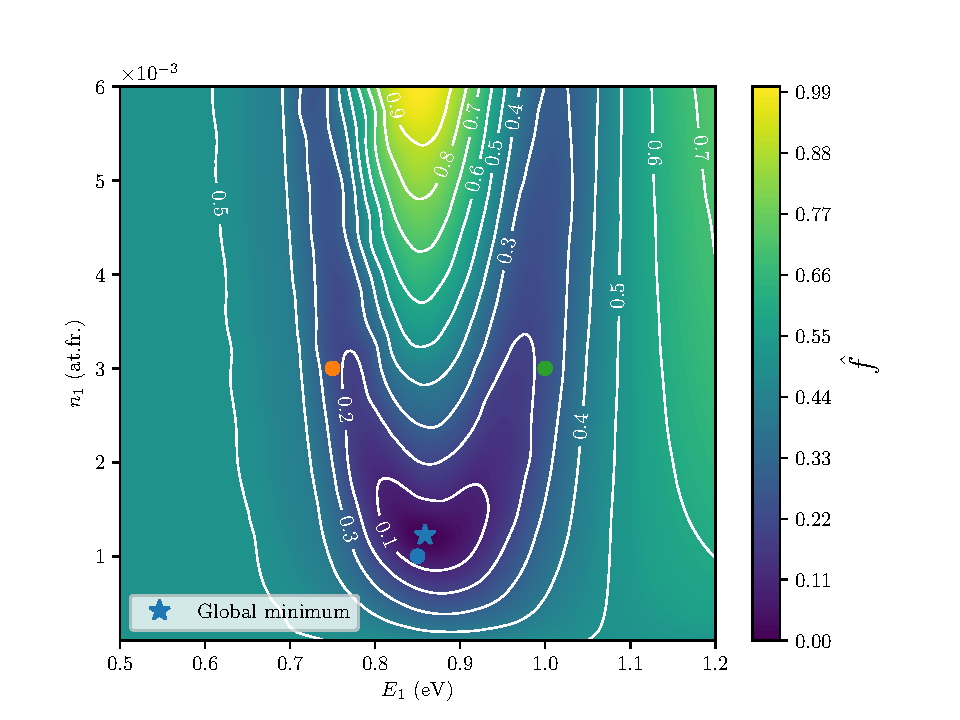
\includegraphics[width=\linewidth]{Figures/Chapter3/Parametric_optimisation/cost_function_2D.pdf}
            \caption{Normalised cost function.}
        \end{subfigure}
        \begin{subfigure}[t]{0.7\linewidth}
            \centering
            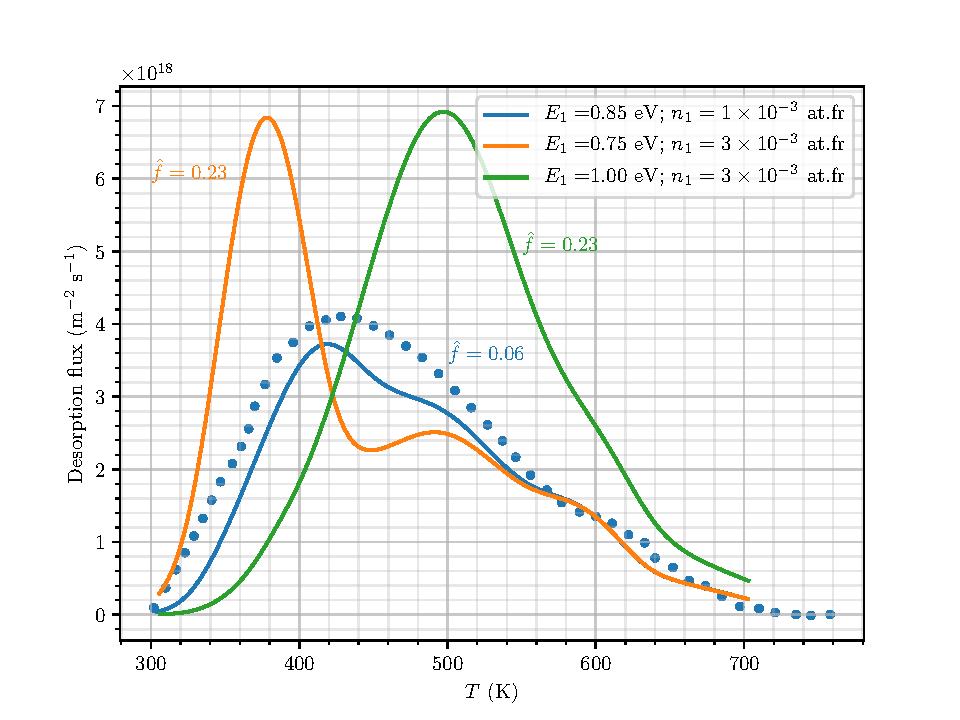
\includegraphics[width=\linewidth]{Figures/Chapter3/Parametric_optimisation/points_on_cost_function.pdf}
            \caption{Corresponding simulated \gls{tds} spectra.}
        \end{subfigure}%
    \caption{Normalised cost function $\hat{f} = (f - \min{f})/(\max{f}-\min{f})$ as function of $E_1$ (\si{eV}) and $n_1$ (\si{at.fr.}) with global minimum located at $(\SI{0.86}{eV}, \SI{1.2e-3}{at.fr.})$.}
    \label{fig:cost function}
\end{figure*}

In this case, when only two free parameters are set the cost function has only one minimum (it is not necessarily the case for higher dimension optimisation problems).
However, if one fixes the trap density $n_1$ above $\approx \SI{2e-3}{at.fr.}$, the cost function has two local minima which can lead the optimisation routine to converged to a non-global minimum.
Moreover, $f$ is smooth and quadratic around its minimum located at $(E_1, n_1) = (\SI{0.86}{eV}, \SI{1.2e-3}{at.fr.})$.
For detrapping energies below \SI{0.6}{eV} and/or densities below \SI{0.5e-3}{at.fr}, the cost function is constant.
This is because for these values, the contribution of this trapping site to the \gls{tds} spectrum is zero either because the density is close to zero, or because the energy is too low for these traps to be filled at the implantation temperature of \SI{300}{K}.
Variations in these regions do not modify the simulated spectrum and thus do not modify the cost function value.

\begin{figure} [ht]
    \centering
    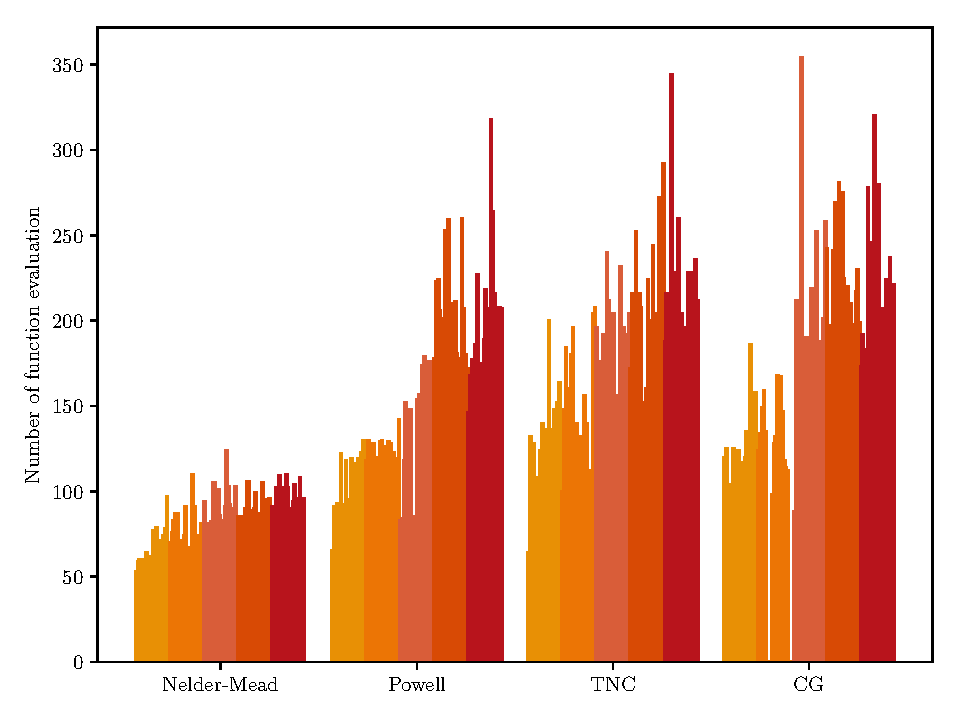
\includegraphics[width=\linewidth]{Figures/Chapter3/Parametric_optimisation/algorithms_perfs.pdf}
    \caption{Number of cost function evaluations required to converge towards the global minimum with 100 different initial guesses sorted by distance to the global minimum for several minimisation algorithms. Each cost function evaluation takes \SI{20}{s} to compute. White stripes correspond to initial guesses for which the algorithm did not converge to the global minimum.}
    \label{fig:algos perfs}
\end{figure}


Four different optimisation algorithms are being compared: 
Nelder-Mead (also called the simplex method), Powell, \gls{tnc} and \gls{cg}.
Thorough descriptions of these algorithms would be beyond the scope of this research but can be found in \sidecite{nocedal_numerical_2006}.
The performances of these algorithms have been compared with 100 different initial guesses randomly distributed on the $(E_1,n_1)$ plane and are shown on Figure \ref{fig:algos perfs}.
It appears that the \gls{cg} algorithm is less robust since for some cases it didn't converge towards the global minimum (see white bands on Figure \ref{fig:algos perfs}).
Nelder-Mead algorithm appears to be the most efficient with initial guesses both close and far from the global minimum since the number of cost function evaluations ranges from 50 to 100 whereas other algorithms require more than 100.
This can be explained by the fact that Nelder-Mead is a derivative-free algorithm whereas \gls{tnc} and \gls{cg} algorithms need on the other hand to compute first order derivatives thus increasing the number of function evaluations.
This will be even more true when increasing the number of free parameters since the derivative will become more costly to compute.

It is worth noting that the Nelder-Mead algorithm is an unconstrained method.
If constraints or bounds are needed, \gls{tnc} might be a more suitable choice.

Though in the following, the Nelder-Mead algorithm will be employed in the following cases.


% \subsubsection{Results} \label{results}

% \subsection{Applications}

% The fitting procedure has been employed to reproduce thermo-desorption experiments performed on Tungsten, EUROFER, Aluminium and Beryllium.


\subsubsection{Validation on tungsten}

The TDS spectrum measured by Ogorodnikova \textit{et al} \sidecite{ogorodnikova_deuterium_2003} has been reproduced by setting all traps parameters as free parameters.
The fitting procedure has been run for several numbers of traps as shown on Figure \ref{fig:number of traps comparison}.
It is clear that setting only one trap is not sufficient to reproduce the experimental data.
The two traps case shows better results but also has a discrepancy near \SI{600}{K}.
This discrepancy is removed when setting a third extrinsic trap to the simulation.

For this last case, the five free parameters are the detrapping energies $E_{p, 1}$, $E_{p, 2}$, $E_{p, 3}$ and densities $n_1$, $n_2$ (the third trapping site being created during the implantation, for which the creation parameters are not part of the free parameters and taken from \cite{ogorodnikova_deuterium_2003} or \sidecite{hodille_macroscopic_2015}).
This optimisation case is therefore a 5D optimisation problem.
Every other parameter is taken from \cite{hodille_macroscopic_2015}.
The resulting fit is shown on Figure \ref{fig:5D TDS} alongside with the contribution of each trap to the total spectrum.
An interesting feature of this spectrum is the negative area of the contribution of the second trap around \SI{400}{K}.
Because not all of these traps are saturated, when trap 1 is empyting, some of the hydrogen particles are nearly instantly trapped in the second trap which has a higher detrapping energy.

% (1 trap [ 0.88368005  1.44347635] 2 traps [ 0.83582125  1.23768655  0.98708714  6.85457283])
\begin{figure*} [h!]
    \centering
        \begin{subfigure}[t]{0.5\linewidth}
            \centering
            \captionsetup{width=.9\linewidth}
            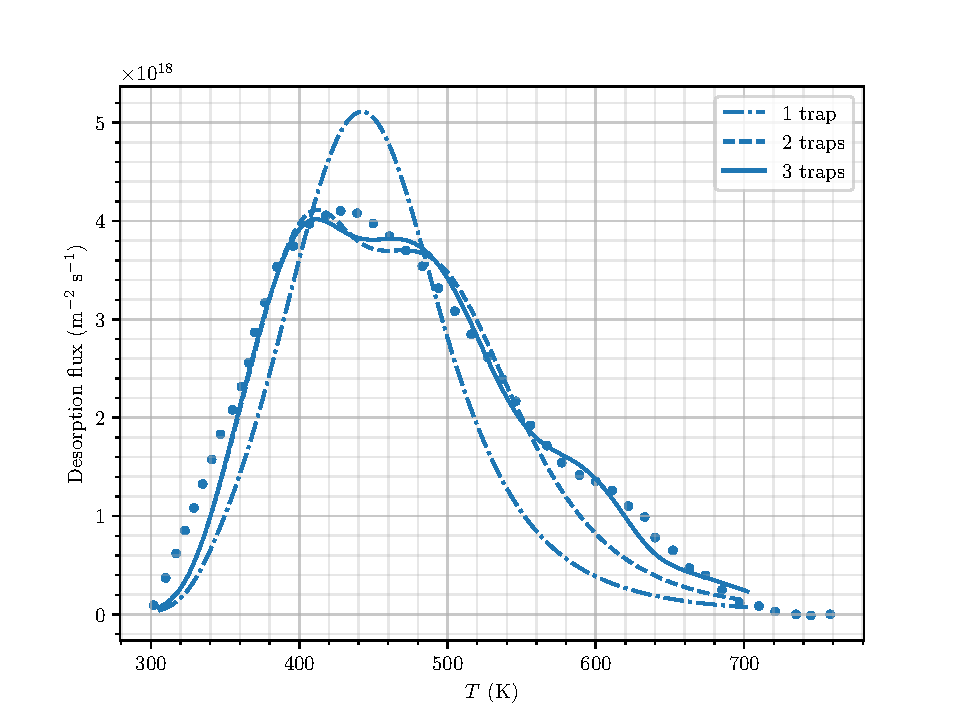
\includegraphics[width=\linewidth]{Figures/Chapter3/Parametric_optimisation/number_of_traps.pdf}
            \caption{Comparison of the resulting fit with several numbers of traps in the simulation.}
            \label{fig:number of traps comparison}
        \end{subfigure}%
        \begin{subfigure}[t]{0.5\linewidth}
            \centering
            \captionsetup{width=.9\linewidth}
            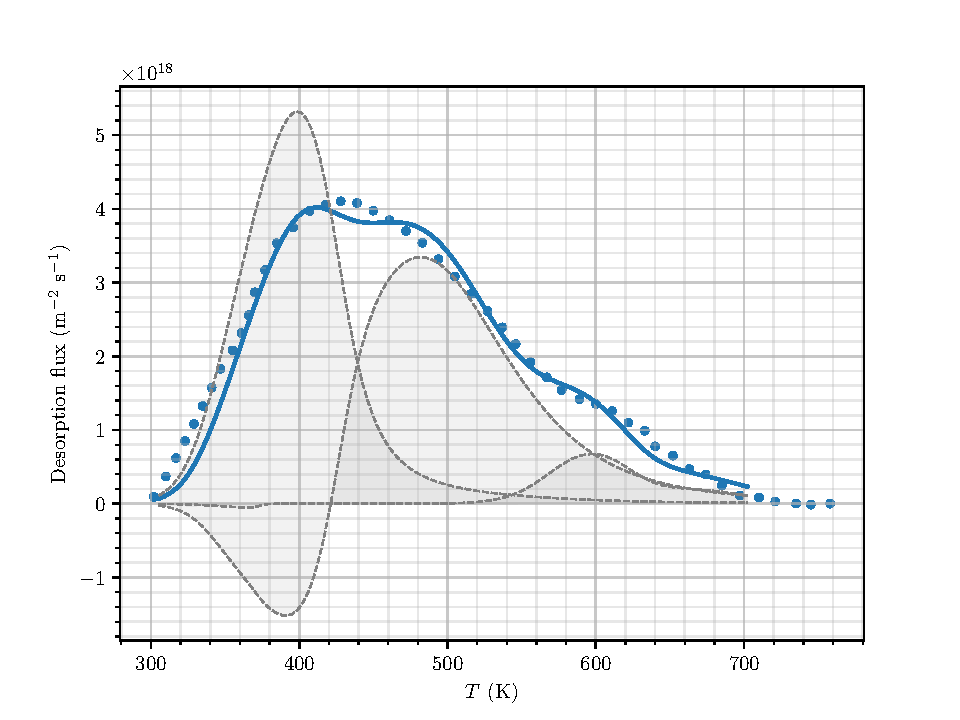
\includegraphics[width=\linewidth]{Figures/Chapter3/Parametric_optimisation/Ogorodnikova_5D.pdf}
            \caption{Identified by the fitting procedure with $E_1 = \SI{0.83}{eV}$, $E_2 = \SI{0.97}{eV}$, $E_3 = \SI{1.51}{eV}$, $n_1 = \SI{1.18e-3}{at.fr.}$ and \newline $n_2 = \SI{7.22e-4}{at.fr.}$.  Dashed lines correspond to the temporal evolution of each trapping population's inventory.}
            \label{fig:5D TDS}
        \end{subfigure}%
    \caption{Fitting TDS spectrum performed on Tungsten by Ogorodnikova \textit{et  al} \cite{ogorodnikova_deuterium_2003}. Dots correspond to experimental data.}
    \label{fig:TDS ogorodnikova}
\end{figure*}
The identified parameters are similar to the ones found by Hodille \textit{et al.} in \cite{hodille_macroscopic_2015}.
The total fitting procedure took a few hundred of cost function evaluations.
One single cost function evaluation "costing" less than \SI{20}{s} to compute (for that specific case), the total procedure lasted less than \SI{3}{h}.

% \subsubsection{EUROFER}

% Hollingsworth \textit{et al} performed thermo-desorption on pre-damaged EUROFER at several damage levels \sidecite{hollingsworth_comparative_2019}.
% Three spectra with similar exposure conditions have been fitted with one trapping site (since only one peak appears on the spectra) as shown on Figure \ref{fig:TDS EUROFER}.

% \begin{figure} [h!]
%     \centering
%     \includegraphics[width=0.9\linewidth]{Figures/Chapter3/Parametric_optimisation/EUROFER_hollingsworth.pdf}
%     \caption{TDS spectra of damaged EUROFER \cite{hollingsworth_comparative_2019}. Fitted with one trapping site (solid line) $E=\SI{1.06}{eV}$ and densities of \SI{8.9e-3}{at.fr}, \SI{2.8e-2}{at.fr} and \SI{5.0e-2}{at.fr} for \SI{0}{dpa}, \SI{0.01}{dpa} and \SI{0.1}{dpa}, respectively. Dashed lines correspond to optimisations with an unweighted cost function. Dots correspond to experimental data.}
%     \label{fig:TDS EUROFER}
% \end{figure}

% To put the emphasis on peaks, a weighting factor of 10 has been applied for $T \in [\SI{445}{K}, \SI{492}{K}]$.
% Not applying this factor near the peak region results in a closer fit in other regions but a higher peak value.
% The identified trap energy is $E_p$ \SI{1.06}{eV} for all spectra whereas the trap density $n$ is \SI{8.9e-3}{at.fr} for the undamaged sample, \SI{2.8e-2}{at.fr} for \SI{0.01}{dpa} and \newline \SI{5.0e-2}{at.fr} for \SI{0.1}{dpa}.
% For all simulations the attempt frequency $p_0$ is \SI{1e13}{s^{-1}} and the diffusion coefficient is taken from \sidecite{esteban_hydrogen_2007}.

% The total fitting procedure took less than two hours for fitting the three spectra.
% A more thorough study of these experiments could involve constraining the algorithm with profilometry data obtained by Hollingsworth \textit{et al} \cite{hollingsworth_comparative_2019}.
% Indeed, having a non-homogeneous trapping site distribution could help having a better fit of both the profilometry data and the TDS spectra. 

% \subsubsection{Aluminium}

% The experiment performed on Aluminium by Quiros \textit{et al} \sidecite{quiros_blistering_2019, quiros_blister_2017} has also been reproduced with FESTIM.

% Only one trap has been set in the simulation and its energy $E_p$ and density $n$ are set as free parameters.
% Every other parameters are fixed and taken from \cite{quiros_blister_2017, quiros_blistering_2019}.
% The resulting simulated TDS spectrum is shown on Figure \ref{fig:TDS alu}.
% \begin{figure} [h!]
%     \centering
%     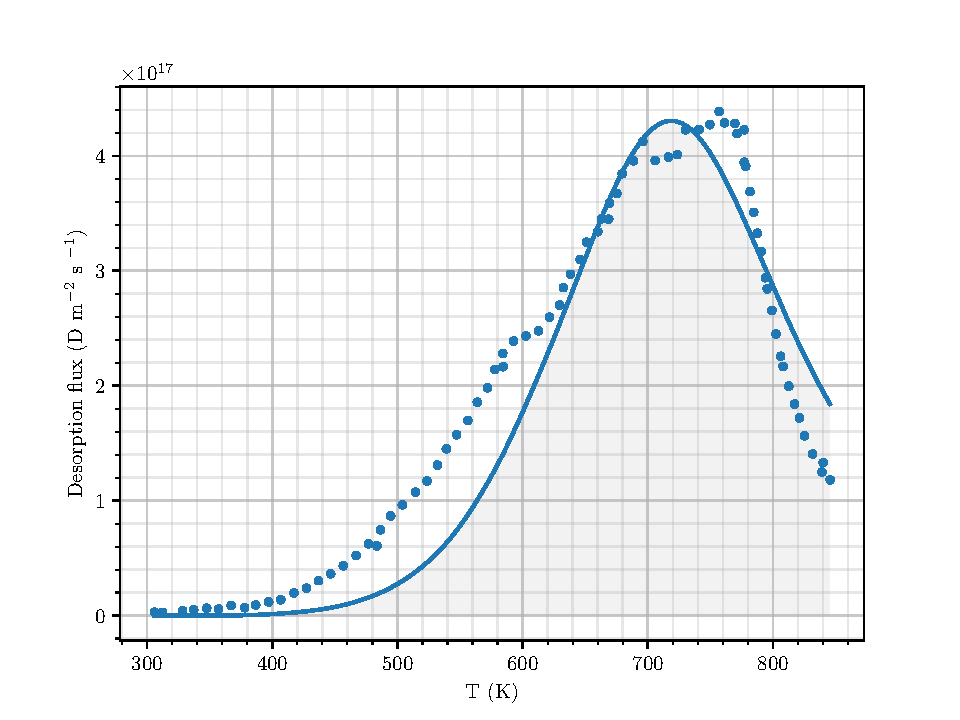
\includegraphics[width=0.9\linewidth]{Figures/Chapter3/Parametric_optimisation/alu_quiros.pdf}
%     \caption{TDS spectrum of aluminium exposed to \SI{3e23}{H.m^{-2}} at \SI{618}{K} \cite{quiros_blister_2017, quiros_blistering_2019}. Fitted with one trapping site $n = \SI{1.8e-2}{at.fr.}$ and $E =\SI{1.1}{eV}$. Dots correspond to experimental data. Dashed lines correspond to the temporal evolution of each trapping population's inventory.}
%     \label{fig:TDS alu}
% \end{figure}


% The identified parameters are $n = \SI{1.8e-2}{at.fr.}$ and $E =\SI{1.1}{eV}$.
% The trapping sites density is significantly higher than the one described in \cite{quiros_blister_2017}.
% However, the TDS spectrum obtained with this procedure better fits the experimental data since the one obtained by Quiros \textit{et al} requires a 10-fold increase.
% The fitting procedure took less than a hundred cost function evaluations, which corresponds in total to a few dozens of minutes.

% \subsubsection{Beryllium}
% Be co-deposition experiments performed by Baldwin \textit{et al} \sidecite{baldwin_experimental_2014} were reproduced.
% In this experiment, a \SI{1}{\micro m} thick Be-D layer is grown on Tungsten at \SI{330}{K}. 
% Following the strategy proposed by Baldwin \textit{et al}, only the thermo-desorption phase has been simulated with two trapping sites with homogeneously distributed densities and with initial occupancies $f_i$.
% There are therefore three free parameters per trap (energy, density and initial occupancy) which makes this optimisation problem 6D.
% It is assumed that the surface flux is the net balance between incoming flux from the chamber (very low since the pressure is $\SI{1}{\micro Pa}$) and the molecular recombination flux.
% All the other parameters are described in \cite{baldwin_experimental_2014}.

% The resulting optimised TDS spectrum is shown on Figure \ref{fig:TDS baldwin}.
% The optimised parameters are $E_{p, 1} = \SI{0.75}{eV}$, $n_1 = \SI{1.09e-1}{at.fr.}$, $f_1=0.73$, $E_{p, 2} = \SI{0.93}{eV}$, \newline ${n_2 = \SI{3.40e-2}{at.fr.}}$, $f_2=0.28$.
% These values are in agreement with the ones found by Baldwin \textit{et al} \cite{baldwin_experimental_2014} and took only a few of minutes to compute since the implantation phase was not simulated.

% \begin{figure} [h!]
%     \centering
%     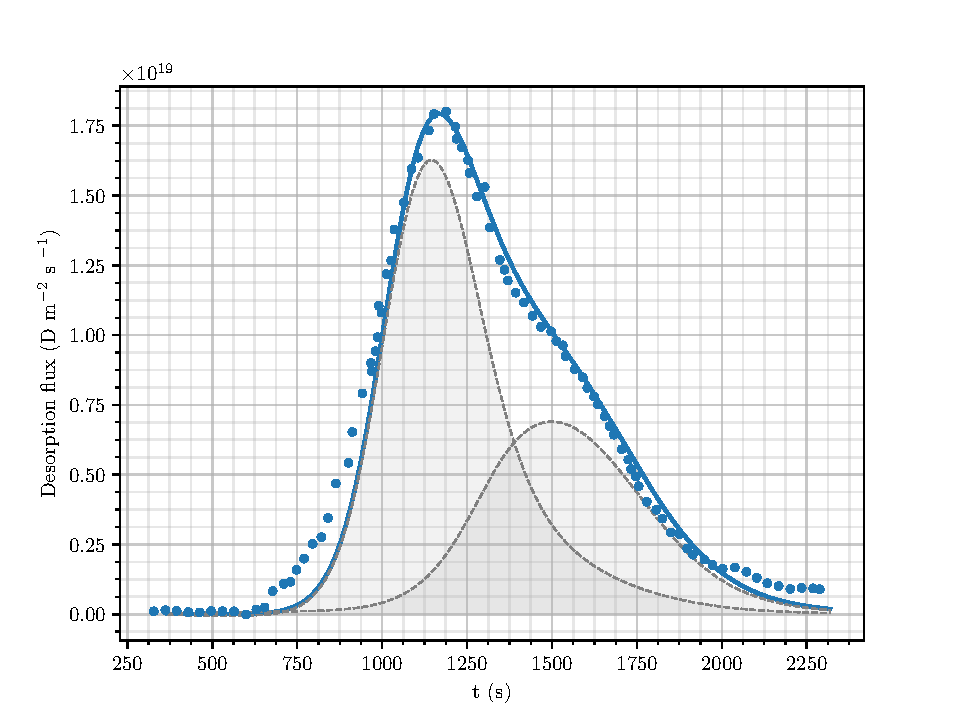
\includegraphics[width=0.9\linewidth]{Figures/Chapter3/Parametric_optimisation/baldwin_be.pdf}
%     \caption{TDS spectrum of co-deposited Be-D \cite{baldwin_experimental_2014} simulated with two trapping sites. Dots correspond to experimental data.}
%     \label{fig:TDS baldwin}
% \end{figure}

\subsubsection{Limitations}

Even though an automated technique is proposed, the user still has some choices to make in order to ensure the credibility of the fitted spectrum.
As shown on Figure \ref{fig:TDS EUROFER}, weighting the cost function near regions of interest will result in a better fit in these regions.
Users should also be aware of the number of traps the data is being fitted with.
As shown on Figure \ref{fig:number of traps comparison} too few traps in the simulation will not result in a satisfactory fit (even though the optimisation routine will converge to an optimised solution).
Moreover, as shown on Figure \ref{fig:hurley_comparison}, one single TDS spectrum can be reproduced with several traps of different energies and densities.
This means that the cost function with several traps as free parameters can have several local minima of very similar values.
Adding traps to an optimisation problem can also help having a better fit of the experimental data in some cases.
But artificially adding more and more traps is not necessarily realistic and could lead to misinterpretation of the results.

\begin{figure}[h!]
    \centering
    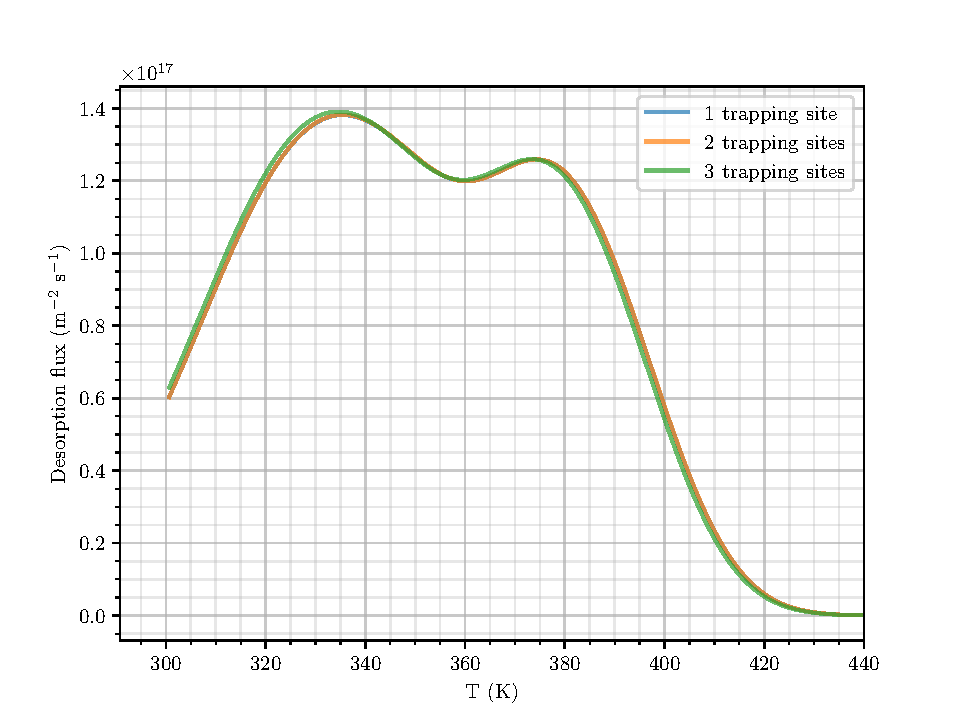
\includegraphics[width=0.9\linewidth]{Figures/Chapter3/Parametric_optimisation/hurley_comparison.pdf}
    \caption{TDS spectrum reproduced with several sets of parameters showing the existence of several solutions to a single optimisation problem.}
    \label{fig:hurley_comparison}
\end{figure}

In the first case with only one trapping site, as described by Hurley \textit{et al} in \sidecite{hurley_numerical_2015}, the binding energy is \SI{0.55}{eV} and the trap density is \SI{2.08e24}{m^{-3}}.
The appearance of two peaks is due to the desorption on different sides of the sample as explained in \cite{hurley_numerical_2015}.
In the second case, the curve as been reproduced with two trapping sites which energies and densities are respectively \SI{0.51}{eV} and \SI{0.57}{eV} and \SI{2.02e24}{m^{-3}} and \SI{2.12e24}{m^{-3}}.
In the third case, it has been reproduced with three trapping sites which energies and densities are respectively \SI{0.55}{eV}, \SI{0.38}{eV} and \SI{0.51}{eV} and \SI{2.12e24}{m^{-3}}, \SI{2.26e24}{m^{-3}} and \newline \SI{2.13e24}{m^{-3}}.

This example illustrates how a single spectrum can be simulated with several sets of parameters by varying the number of traps in the simulation.
One way to avoid this from happening is to have a set of experiments with varying parameters such as the implantation temperature, the heating ramp, the fluence, dwelling time before TDS, etc.


\subsection{Comparison with TMAP7}

The FESTIM code was compared to TMAP7 \sidecite{longhurst_tmap7_2008} on a 1D case.

The 1D simulation case is a \SI{8.5}{mm}-thick composite slab made of W, Cu and CuCrZr (see \reffig{monoblock 1D geometry}).
The plasma facing surface $\Gamma_\mathrm{top}$ is located at $x=\SI{0}{mm}$ and the surface cooled by water $\Gamma_\mathrm{coolant}$ is located at $x=\SI{8.5}{mm}$.
The trapping parameters are detailed in \reftab{traps comparison tmap}.
The boundary conditions are detailed in \refeq{code comparison BCs}.

\begin{figure}
    \begin{overpic}[width=0.75\linewidth]{Figures/Chapter3/monoblocks/interface_condition/iter case/Monoblock 1D.pdf}
        \put(40, 50){\SI{6}{mm}}
        \put(40, 8){W}
        \put(62, 50){\SI{1}{mm}}
        \put(65, 8){Cu}
        \put(72, 50){\SI{1.5}{mm}}
        \put(72, 8){CuCrZr}
        \put(6, 25){\large$\Gamma_\mathrm{top}$}
        \put(85, 25){\large$\Gamma_\mathrm{coolant}$}
    \end{overpic}
    \caption{TMAP7 - FESTIM comparison 1D geometry showing W \cruleme[grey]{0.3cm}{0.3cm}, Cu \cruleme[orange]{0.3cm}{0.3cm}, CuCrZr \cruleme[yellow]{0.3cm}{0.3cm}.}
    \labfig{monoblock 1D geometry}
\end{figure}

\begin{table*}
    \centering
    \begin{tabular}{L{1.5cm} L{1.5cm} R{1.7cm} R{1.1cm} R{1.6cm} R{1.1cm} R{1.9cm}}
         & Material & $k_0 (\si{m^3.s^{-1}})$ &  $E_k (\si{eV})$ & $p_0 (\si{s^{-1}})$ & $E_p (\si{eV})$ & $n_i (\si{at.fr.})$ \\
        \hline
        \\
        Trap 1 & W & $3.8 \times 10^{-17}$ & 0.39 & $8.4 \times 10^{12}$& 1.20 & $5.0 \times 10^{-4}$ \\
        \\
        Trap 2 & W & $3.8 \times 10^{-17}$ & 0.39 & $8.4 \times 10^{12}$& 1.40 & $5.0 \times 10^{-3}$ \\
        \\
        Trap 3 & Cu & $6.0 \times 10^{-17}$ & 0.39 & $8.0 \times 10^{13}$ & 0.50 &$5.0 \times 10^{-5}$\\
        \\
        Trap 4 & CuCrZr & $1.2\times 10^{-16}$ & 0.42 & $8.0 \times 10^{13}$ & 0.50 &$5.0 \times 10^{-5}$\\
        \\
        Trap 5 & CuCrZr & $1.2\times 10^{-16}$ & 0.42 & $8.0 \times 10^{13}$ & 0.83 &$4.0 \times 10^{-2}$\\
        \\
    \end{tabular}
    \caption{Traps properties used in the comparison with TMAP7.}
    \labtab{traps comparison tmap}
\end{table*}

\begin{subequations}
    \begin{align}
    T &= \SI{1200}{K}\quad \text { on } \Gamma_\mathrm{top}\\
    c_\mathrm{m} &=  \frac{\varphi_\mathrm{imp} \cdot R_p}{D} \quad \text { on } \Gamma_\mathrm{top}\\
    T &= \SI{373}{K} \quad \text { on } \Gamma_\mathrm{coolant}\\
    -D \nabla c_\mathrm{m} \cdot \mathbf{n} &= K_\mathrm{CuCrZr} \cdot c_\mathrm{m}^{2} \quad \text { on } \Gamma_\mathrm{coolant}  
    \end{align}
    \labeq{code comparison BCs}
\end{subequations}
% $\varphi_\mathrm{imp} = \SI{5e23}{m^{-2}.s^{-1}}$ the implanted particle flux, $R_p = \SI{1.25}{nm}$ the implantation depth, $\mathbf{n}$ the normal vector and 
with $K_{r,\mathrm{CuCrZr}} = 2.9 \times 10^{-14}\cdot \exp{(-1.92/(k_B\cdot T))}$ the recombination coefficient of the CuCrZr (in vacuum) expressed in \si{m^4.s^{-1}} \sidecite{anderl_deuterium_1999}.

The Dirichlet boundary condition on $\Gamma_\mathrm{top}$ for the hydrogen transport corresponds to a flux balance between the implanted flux and the flux that is retro-desorbed at the surface (see \refsec{triangle model}).
The temperature profile in TMAP7 was fixed on the temperature profile produced by FESTIM (see \reffig{temperature}).

TMAP7 and FESTIM were found to be in very good agreement (see \reffig{code comparison}).

\begin{figure*} [h]
    \centering
    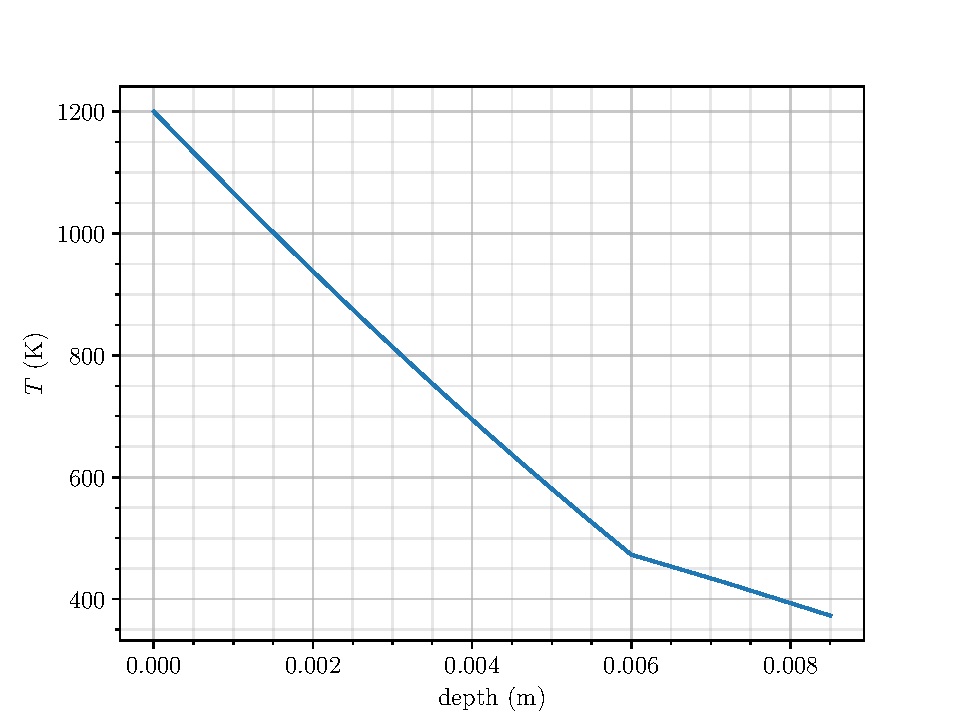
\includegraphics[width=0.5\linewidth]{Figures/Chapter3/monoblocks/interface_condition/iter case/temperature_1D.pdf}
    \caption{Temperature profile simulated by FESTIM for comparison case with TMAP7.}
    \labfig{temperature}
\end{figure*}

\begin{figure} [h]
    \centering
    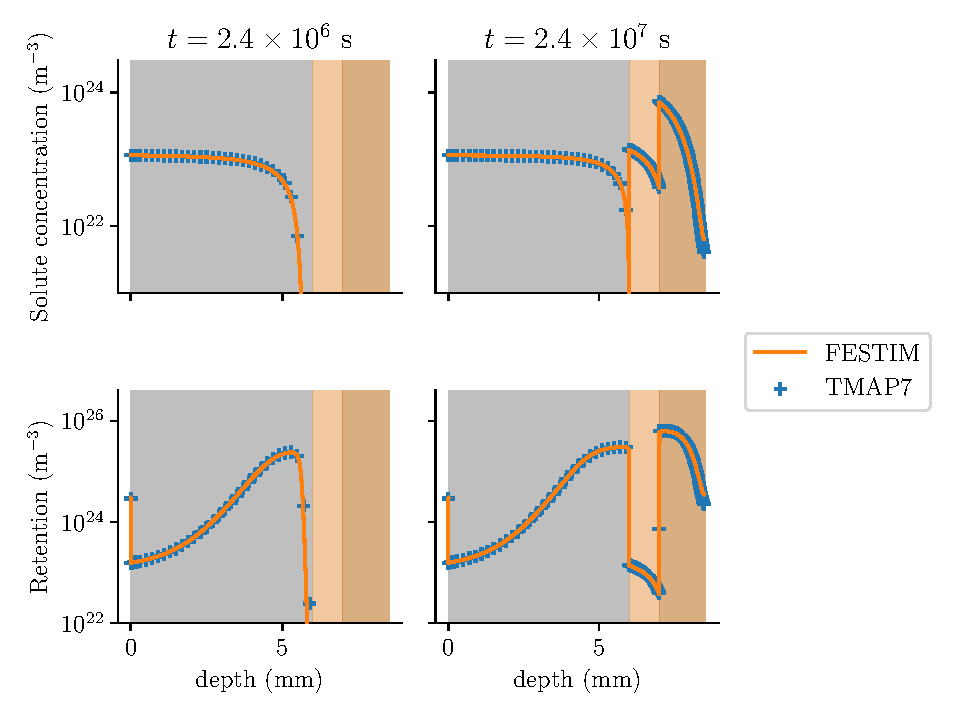
\includegraphics[width=\linewidth]{Figures/Chapter3/monoblocks/interface_condition/iter case/comparison_codes.pdf}
    \caption{Comparison of results provided by FESTIM and TMAP7.}
    \labfig{code comparison}
\end{figure}



\section{Summary}

The macroscopic rate equations model describing the transport (diffusion and trapping) of H in solids was presented alongside with additional models such as the conservation of chemical potential at interfaces.
Due to the presence of thermally activated processes (diffusion, trapping, detrapping, surface processes, ...), the heat transfer equation has to be solved numerically.
All these equations are solved with the finite element code FESTIM, which heavily relies of FEniCS.

FESTIM has been verified using methods such as the Method of Exact Solutions and the Method of Manufactured Solutions.
On the other hand, it was shown that FESTIM could be employed to reproduce real-life experiments (TDS experiments) performed on Tungsten, Aluminium, Beryllium and EUROFER.
This validation process could be extended by reproducing other types of experiments such as permeation experiments and profilometry.
However, this set of equation (shared amongst H transport codes) has already proven to be capable of reproducing these experiments.
This has been done, for instance, during the validation of TMAP7 \sidecite{longhurst_tmap7_2008}.

Thanks to this verification \& validation process, it was shown that (1) the governing equations were correctly solved and (2) these equations can represent real life processes.

The FESTIM code can then be safely employed to perform analysis on tokamak components.
